\documentclass{article}
\usepackage[utf8]{inputenc}
\usepackage{graphicx}
\usepackage{hyperref}
\usepackage{titling}
\usepackage{array}
\usepackage{enumitem}
\usepackage{listings}
\usepackage{xcolor}
\usepackage{geometry}
\usepackage{amsmath}
\usepackage{amssymb}
\usepackage{titlesec}
\usepackage{pgfgantt}

% Float management
\usepackage{float}        % Allows [H] specifier
\usepackage{placeins}     % For \FloatBarrier
\usepackage{tabularx}     % Auto-wrap columns
\usepackage{adjustbox}    % For scaling large content (flowcharts, etc.)
\usepackage{booktabs}

% --- TikZ and PGF for flowcharts ---
\usepackage{tikz}
\usetikzlibrary{shapes.geometric, arrows}
\usepackage{minted}
\usepackage[T1]{fontenc}

\geometry{a4paper, margin=1in}

\setcounter{secnumdepth}{4}
\setcounter{tocdepth}{4} 

\titleformat{\paragraph}
{\normalfont\normalsize\bfseries}{\theparagraph}{1em}{}
\titlespacing*{\paragraph}
{0pt}{3.25ex plus 1ex minus .2ex}{1.5ex plus .2ex}

\definecolor{codebg}{rgb}{0.95,0.95,0.95}
\definecolor{keywordblue}{RGB}{33,33,255}
\definecolor{commentgray}{RGB}{85,85,85}
\definecolor{stringorange}{rgb}{0.71,0.22,0.05}

% Define a custom "Pseudo" language for listings
\lstdefinelanguage{Pseudo}{
  % Recognized keywords (add as needed)
  morekeywords={
    FUNCTION,END,ENDFUNCTION,ENDFUNCTION,
    IF,THEN,ELSE,ELIF,ENDIF,
    WHILE,ENDWHILE,
    FOR,ENDFOR,
    SWITCH,CASE,DEFAULT,BREAK,
    RETURN,RAISE_ERROR,PRINT,
    CREATE,INITIALIZE,
    ADD,REMOVE,REGISTER,PROCESS,UPDATE,TERMINATE,
    LOGOUT,
    ASSIGN_THREAD,START_THREAD,
    REPLENISH_ELIXIR
  },
  sensitive=false, 
  comment=[l]{\#},
  morecomment=[s]{/*}{*/},
  morestring=[b]"
}

\lstdefinestyle{pseudo}{
  language=Pseudo,                         % use our custom language
  backgroundcolor=\color{codebg},          % set background color
  basicstyle=\small\ttfamily,              % base font style
  keywordstyle=\bfseries\color{keywordblue},% style of keywords
  commentstyle=\itshape\color{commentgray},% style of comments
  stringstyle=\color{stringorange},        % style of strings
  frame=single,                            % box around the code
  rulecolor=\color{black},
  numbers=left,                            % line numbers on the left
  numberstyle=\tiny\color{commentgray},    % line number style
  stepnumber=1,
  numbersep=6pt,
  showstringspaces=false,
  breaklines=true,
  columns=fullflexible,
  tabsize=4,
  keepspaces=true
}

\tikzstyle{startstop} = [rectangle, rounded corners, minimum width=2.5cm, minimum height=0.8cm, text centered, draw=black, fill=gray!20]
\tikzstyle{io} = [trapezium, trapezium left angle=70, trapezium right angle=110, minimum width=2.8cm, minimum height=0.8cm, text centered, draw=black, fill=blue!20]
\tikzstyle{process} = [rectangle, minimum width=2.8cm, minimum height=0.8cm, text centered, draw=black, fill=orange!20]
\tikzstyle{decision} = [diamond, aspect=2, text centered, draw=black, fill=green!20]
\tikzstyle{arrow} = [thick,->,>=stealth]

\title{Clash Royale Online Implementation}
\author{Paul Hodges}
\date{\today}

\begin{document}

\begin{titlepage}
    \centering
    \vspace*{4cm}
    {\Huge \textbf{Clash Royale} \par}
    \vspace{2cm}
    {\Large by \par}
    \vspace{1cm}
    {\Large Paul Hodges \par}
    \vspace{3cm}
    {\Large \today \par}
    \vspace*{4cm}
\end{titlepage}

\tableofcontents
\newpage

\section{Development Schedule}

\subsection{Planning and Documentation}
\begin{ganttchart}[
    hgrid,
    vgrid={*{4}{gray, dotted}, *1{black, dashed}},
    bar label node/.append style={align=left},
    bar/.append style={fill=blue!40},
    group/.append style={fill=blue!20},
    milestone/.append style={fill=red, inner sep=2pt},
    title label font=\bfseries\footnotesize,
    bar label font=\footnotesize,
    y unit chart=0.5cm,
    x unit=10pt,
    canvas/.style={draw=none, fill=none},
    progress label node/.append style={below right=10pt},
    link/.style={->, thick, rounded corners=2pt},
    title/.style={draw=none, fill=white},
    title label node/.append style={below=0pt},
    title height=0.75,
    bar height=0.6,
    milestone height=0.6,
    group top shift=0.5,
    group height=0.2
]{1}{28}
\gantttitle{Week 1}{7} \gantttitle{Week 2}{7} \gantttitle{Week 3}{7} \gantttitle{Week 4}{7} \\

\ganttgroup[group/.append style={fill=blue!20}]{Phase 1: Planning \& Documentation}{1}{28} \\

    % Requirements and Design
    \ganttbar[bar/.append style={fill=blue!50}]{Project Scope Definition}{1}{4} \\
    \ganttbar[bar/.append style={fill=blue!50}]{Game Rules and Mechanics Research}{5}{8} \\
    \ganttbar[bar/.append style={fill=blue!50}]{Requirement Specification}{9}{12} \\
    \ganttbar[bar/.append style={fill=blue!50}]{Functional \& Non-Functional Requirements}{13}{15} \\
    \ganttmilestone[milestone/.append style={fill=red}]{Requirements Finalized}{15} \\

    % System Design
    \ganttbar[bar/.append style={fill=blue!50}]{System Architecture Design}{16}{18} \\
    \ganttbar[bar/.append style={fill=blue!50}]{Networking Protocol Design}{19}{21} \\
    \ganttbar[bar/.append style={fill=blue!50}]{ECS (Entity Component System) Structure}{22}{24} \\
    \ganttbar[bar/.append style={fill=blue!50}]{Game State Synchronization}{25}{26} \\
    \ganttmilestone[milestone/.append style={fill=red}]{System Design Complete}{26} \\

    % Algorithm Development
    \ganttbar[bar/.append style={fill=blue!50}]{Flowchart Creation}{16}{20} \\
    \ganttbar[bar/.append style={fill=blue!50}]{Pseudocode for Core Systems}{21}{23} \\
    \ganttbar[bar/.append style={fill=blue!50}]{Finalizing Planning Document}{27}{28} \\
    \ganttmilestone[milestone/.append style={fill=red}]{Planning Document Complete}{28} \\

\end{ganttchart}

\subsection{Programming and Development}
\begin{ganttchart}[
    hgrid,
    vgrid={*{4}{gray, dotted}, *1{black, dashed}},
    bar label node/.append style={align=left},
    bar/.append style={fill=green!40},
    group/.append style={fill=green!20},
    milestone/.append style={fill=red, inner sep=2pt},
    title label font=\bfseries\footnotesize,
    bar label font=\footnotesize,
    y unit chart=0.5cm,
    x unit=10pt,
    canvas/.style={draw=none, fill=none},
    progress label node/.append style={below right=10pt},
    link/.style={->, thick, rounded corners=2pt},
    title/.style={draw=none, fill=white},
    title label node/.append style={below=0pt},
    title height=0.75,
    bar height=0.6,
    milestone height=0.6,
    group top shift=0.5,
    group height=0.2
]{29}{56}
\gantttitle{Week 5}{7} \gantttitle{Week 6}{7} \gantttitle{Week 7}{7} \gantttitle{Week 8}{7} \\

\ganttgroup[group/.append style={fill=green!20}]{Phase 2: Programming \& Development}{29}{56} \\

    % Core Engine Development
    \ganttbar[bar/.append style={fill=green!50}]{ECS System Implementation}{29}{32} \\
    \ganttbar[bar/.append style={fill=green!50}]{Rendering System (2D/3D Hybrid)}{33}{35} \\
    \ganttmilestone[milestone/.append style={fill=red}]{Core Engine Ready}{35} \\

    % Networking
    \ganttbar[bar/.append style={fill=green!50}]{Server-Client Communication}{36}{38} \\
    \ganttbar[bar/.append style={fill=green!50}]{Binary Protocol Implementation}{39}{40} \\
    \ganttmilestone[milestone/.append style={fill=red}]{Networking Ready}{40} \\

    % Gameplay Mechanics
    \ganttbar[bar/.append style={fill=green!50}]{Card System \& Deck Management}{41}{43} \\
    \ganttbar[bar/.append style={fill=green!50}]{Real-time Battle Logic}{44}{46} \\
    \ganttbar[bar/.append style={fill=green!50}]{Tower AI and Targeting}{47}{48} \\
    \ganttmilestone[milestone/.append style={fill=red}]{Core Gameplay Functional}{48} \\

    % Testing and Debugging
    \ganttbar[bar/.append style={fill=green!50}]{Unit Testing (Game Logic)}{49}{51} \\
    \ganttbar[bar/.append style={fill=green!50}]{Multiplayer Testing}{52}{53} \\
    \ganttbar[bar/.append style={fill=green!50}]{Final Debugging \& Optimization}{54}{55} \\
    \ganttmilestone[milestone/.append style={fill=red}]{Development Complete}{56} \\

\end{ganttchart}

\section{Problem Outline}

The purpose of this project is to develop a simplified but functional online version of Clash Royale using Python. This real-time strategy game implementation will focus on core gameplay mechanics and network functionality, demonstrating practical software development skills in a gaming context.

\noindent The game will allow players to:
\begin{itemize}
    \item Engage in real-time, online strategic battles against other players
    \item Build and customize card decks from their collection
    \item Progress through a skill-based arena system
    \item Earn rewards through a chest system to expand their card collection
    \item Experience the core strategic elements that make Clash Royale engaging
\end{itemize}

\noindent This implementation serves as both an educational tool for understanding game development principles and a demonstration of networking, database management, and software architecture skills in a cohesive application.

\section{Problem Description}

\subsection{Game Overview}
Clash Royale is a \textbf{fast-paced, real-time strategy} (RTS) game that incorporates elements from multiple genres:

\begin{itemize}
    \item \textbf{Collectible Card Game (CCG):} Players build and customize decks from a pool of collectible cards. Each card corresponds to a troop, spell, or building, each with its own unique attributes and effects.
    \item \textbf{Tower Defense:} Players must defend their own towers (two Princess Towers and one King Tower) from enemy attacks while simultaneously attempting to destroy opponent towers.
    \item \textbf{Multiplayer Online Battle Arena (MOBA):} Two players face off in a real-time battle, managing resources (elixir) and positioning units tactically on a symmetrical arena.
\end{itemize}

Key aspects include:
\begin{itemize}
    \item \textbf{Short Match Durations:} Standard matches last 3 minutes, potentially extended by sudden-death overtime.
    \item \textbf{Focus on Tactics and Timing:} Players must carefully manage elixir and deploy units at optimal moments.
    \item \textbf{Intense Head-to-Head Combat:} Each battle is a direct confrontation with another human opponent.
\end{itemize}

\subsection{Game Objectives}
\begin{itemize}
    \item \textbf{Primary Goal:} Destroy more towers than the opponent before time runs out, or immediately win by destroying the enemy King Tower.
    \item \textbf{Crown System:}
    \begin{itemize}
        \item Destroying a Princess Tower yields 1 crown.
        \item Destroying the King Tower yields 3 crowns, resulting in an instant victory.
    \end{itemize}
    \item \textbf{Overtime:} If both players have an equal number of crowns at the end of 3 minutes, the match enters a sudden-death overtime (up to 2 minutes). The first player to gain a lead in crowns during overtime wins immediately.
    \item \textbf{Draw:} If neither player gains an advantage by the end of overtime, the match ends in a draw.
\end{itemize}

\subsection{Core Game Rules}
\begin{enumerate}[label=\arabic*.]
    \item \textbf{Deck and Card Mechanics:}
    \begin{itemize}
        \item Each player prepares an \textbf{8-card deck} to bring into a match.
        \item At the start of a match, players see \textbf{4 random cards} from their deck.
        \item Once a card is played, it is immediately replaced from the remaining deck cards to maintain a 4-card hand.
        \item Cards have different rarities (Common, Rare, Epic, Legendary) and can be upgraded to increase stats.
    \end{itemize}

    \item \textbf{Elixir Resource:}
    \begin{itemize}
        \item Elixir is the primary resource used to deploy cards. 
        \item Elixir regenerates at a base rate of \textbf{1 elixir per 2.8 seconds}.
        \item The maximum elixir capacity is \textbf{10 units}.
        \item During the first minute of overtime, elixir generation doubles (about 1 elixir per 1.4 seconds), and it can triple in the second minute (about 1 elixir per 0.9 seconds), depending on the game mode.
    \end{itemize}

    \item \textbf{Deployment Rules:}
    \begin{itemize}
        \item Troops and buildings must generally be deployed on the player's side of the arena.
        \item Certain spells can be deployed anywhere (e.g., damage spells) as allowed by individual card mechanics.
        \item Cards cannot be deployed if the player does not have enough elixir; partial elixir usage is not possible.
    \end{itemize}

    \item \textbf{Unit Behavior:}
    \begin{itemize}
        \item Troops move automatically toward enemy units or towers following predefined paths, typically targeting the nearest threat or specific priority targets (e.g., building-focused troops).
        \item Air and ground units have separate movement planes, meaning air troops may bypass ground-only defenses if not countered by anti-air.
        \item Troops have attributes such as health, damage per second (DPS), movement speed, attack speed, attack range, and special abilities (e.g., area damage).
    \end{itemize}

    \item \textbf{Match Duration and Victory:}
    \begin{itemize}
        \item The standard match duration is \textbf{3 minutes}.
        \item If the crowns are tied after 3 minutes, \textbf{overtime} begins with sudden-death rules.
        \item Destroying an opponent’s King Tower results in an immediate victory regardless of time or remaining towers.
    \end{itemize}
\end{enumerate}

\subsection{Gameplay Flow}
\begin{enumerate}[label=\arabic*.]
    \item \textbf{Matchmaking:}
    \begin{itemize}
        \item Players are paired based on trophy count, ensuring comparable skill levels (within acceptable matchmaking ranges).
        \item Additional factors (e.g., hidden matchmaking rating, player level) can be considered to improve match quality.
    \end{itemize}

    \item \textbf{Battle Start:}
    \begin{itemize}
        \item Each player begins with around \textbf{5 elixir} (default) and 4 randomly drawn cards from their 8-card deck.
        \item A short \textbf{countdown} (e.g., 3 seconds) precedes the start of the match, allowing players to view their starting hand.
    \end{itemize}

    \item \textbf{Real-Time Combat:}
    \begin{itemize}
        \item Players deploy troops, buildings, or spells using elixir. 
        \item Units spawn at the chosen deployment location and automatically engage enemy targets.
        \item Spell effects apply immediately if valid (e.g., damage, stun, or buff).
    \end{itemize}

    \item \textbf{Tower Destruction:}
    \begin{itemize}
        \item When a tower's HP reaches zero, it is destroyed. The opposing player gains crowns accordingly.
        \item Destruction of the King Tower instantly ends the match with a 3-crown victory for the attacker.
    \end{itemize}

    \item \textbf{Overtime and Conclusion:}
    \begin{itemize}
        \item If crowns are tied at the end of regulation, the match enters \textbf{overtime}.
        \item Elixir generation rate may \textbf{double or triple} during overtime for faster-paced final engagements.
        \item If the tie persists after overtime, the match concludes in a \textbf{draw}.
        \item Players are shown a \textbf{results screen} detailing crowns, trophies gained/lost, and any rewards.
    \end{itemize}
\end{enumerate}

\subsection{Scoring System}
\begin{itemize}
    \item \textbf{Princess Tower Destruction:} +1 crown per destroyed Princess Tower.
    \item \textbf{King Tower Destruction:} +3 crowns; match ends immediately.
    \item \textbf{Time Expiration:} If no King Tower is destroyed, the player with the most crowns wins.
    \item \textbf{Draw:} If the match remains tied after overtime, both players neither gain nor lose trophies (in most modes).
    \item \textbf{Trophy Adjustment:} Winners gain trophies; losers lose trophies. Draws typically result in no or minimal trophy change.
\end{itemize}

\subsection{Winner Determination}
\begin{itemize}
    \item \textbf{Instant Victory:} Destroying the opponent’s King Tower at any time.
    \item \textbf{Crown Comparison:} If neither King Tower is destroyed, the number of Princess Towers destroyed determines the winner.
    \item \textbf{Overtime Mechanic:} Sudden death rules apply, where the next destroyed tower (or difference in crowns) decides the match outcome.
    \item \textbf{Draw:} If neither player secures a lead by the end of overtime, the match is declared a draw.
\end{itemize}

\subsection{Advanced Game Mechanics and Strategies}
\begin{itemize}
    \item \textbf{Elixir Management:} Maintaining a balance between offense and defense, ensuring players do not overspend or waste potential elixir generation.
    \item \textbf{Counter Deployment:} Identifying key counters for popular units (e.g., swarm troops counter single-target tanks, ranged troops counter slow-moving units, etc.).
    \item \textbf{Card Synergies:} Combining cards (e.g., tank + high-DPS unit) for effective pushes. Air-ground synergy is particularly important.
    \item \textbf{Lane Pressure:} Forcing opponents to split their defenses by attacking both left and right lanes strategically.
    \item \textbf{Elixir Counting:} Skilled players track the approximate elixir of the opponent to gauge when to launch a heavy push.
    \item \textbf{Card Cycle Management:} Players cycle quickly to return to \textbf{core cards} (win conditions or essential counters).
    \item \textbf{Tower Trading:} Allowing a weaker tower to fall can free elixir for a stronger, faster offensive counter-push.
    \item \textbf{Spell Value:} Using damaging spells to hit multiple units at once, or a unit plus a tower, maximizes elixir efficiency.
    \item \textbf{Unit Placement:} Subtle differences in troop deployment positions can dramatically change the outcome of an interaction (kiting, path manipulation).
    \item \textbf{Timing:} Well-timed deployments catch opponents low on elixir or out of defensive options, leading to big elixir swings.
\end{itemize}

\newpage

\section{Requirements}

\subsection{Functional Requirements}

\begin{enumerate}[label=\textbf{FR\arabic*.}]

\item \textbf{Server-Client Architecture}
\begin{itemize}
    \item \textbf{Real-Time Multiplayer Connection:}
    \begin{itemize}
        \item The system shall use a \textbf{persistent connection protocol} (e.g., WebSockets) to ensure minimal latency and real-time data exchange.
        \item Each client connection shall be \textbf{encrypted} (e.g., TLS/SSL) to protect sensitive information.
    \end{itemize}
    \item \textbf{Centralized Game Logic:}
    \begin{itemize}
        \item The server shall manage all core gameplay elements (e.g., elixir ticks, card interactions, damage calculations) for fairness and anti-cheat purposes.
        \item Clients shall send deployment/spell actions, and the server shall validate and execute these actions within game state updates.
    \end{itemize}
    \item \textbf{Scalability and Load Balancing:}
    \begin{itemize}
        \item The architecture must allow horizontal scaling with load balancers to distribute matchmaking requests and battle servers as the player base grows.
        \item A \textbf{master server} may handle matchmaking, while additional \textbf{battle servers} simulate individual matches.
    \end{itemize}
    \item \textbf{Connection Handling:}
    \begin{itemize}
        \item The system must manage client \textbf{disconnections} gracefully, allowing rejoin within a defined grace period (e.g., 30 seconds).
        \item Idle sessions shall be terminated to free server resources.
    \end{itemize}
\end{itemize}

\item \textbf{Card Management System}
\begin{itemize}
    \item \textbf{Card Collection:}
    \begin{itemize}
        \item Each player has a \textbf{personal inventory} of collected cards, stored and displayed in a dedicated UI (e.g., ``Card Collection'' screen).
        \item Cards are grouped by rarity (Common, Rare, Epic, Legendary) and may also be sorted by elixir cost, usage frequency, or level.
    \end{itemize}
    \item \textbf{Deck Building:}
    \begin{itemize}
        \item Players must be able to \textbf{create, edit, and save multiple decks} of exactly 8 cards.
        \item The deck-building interface shall validate that the deck has no illegal combinations if such constraints exist (e.g., no duplicates in standard modes).
        \item Players shall have the option to \textbf{rename} their decks for quick identification.
    \end{itemize}
    \item \textbf{Card Upgrades:}
    \begin{itemize}
        \item Each card has \textbf{level-based} attributes. Upgrades require gold and a certain number of card copies.
        \item Players shall receive a notification or prompt when they have enough copies and gold to perform an upgrade.
        \item Upgrading a card increases \textbf{hitpoints, damage, or other relevant stats} depending on the card type.
    \end{itemize}
    \item \textbf{Card Unlocking:}
    \begin{itemize}
        \item New cards become available as players reach certain \textbf{trophy thresholds} (arena levels).
        \item Players can obtain these cards through \textbf{chests}, shop purchases (if implemented), or special events.
    \end{itemize}
\end{itemize}

\item \textbf{Real-time Battle Simulation}
\begin{itemize}
    \item \textbf{Game State Updates:}
    \begin{itemize}
        \item The server shall send synchronized updates (positions, health, elixir, etc.) at a rate of at least \textbf{10 ticks per second}.
        \item Clients shall interpolate or render the game state for smooth animations on the front end.
    \end{itemize}
    \item \textbf{Deployment and Combat Resolution:}
    \begin{itemize}
        \item Each deployment request from the client must include \textbf{card ID, position, and current elixir count}. 
        \item The server validates and executes the deployment if the player has sufficient elixir and the placement is valid.
        \item Combat is automatically resolved by the server, computing \textbf{damage} based on unit stats, interactions, and spells.
    \end{itemize}
    \item \textbf{Collisions and Pathfinding:}
    \begin{itemize}
        \item The system shall implement a simplified pathfinding algorithm to prevent units from occupying the same space. 
        \item If two units meet head-on, one or both may adjust pathing slightly to avoid overlap, or a priority system may determine which unit yields ground.
    \end{itemize}
    \item \textbf{Overtime Mechanics:}
    \begin{itemize}
        \item Once regulation time ends in a tie, the system triggers \textbf{sudden death} and adjusts the elixir regeneration rate.
        \item If a tower is destroyed during sudden death, the match ends instantly.
        \item If the tie persists after the defined overtime period, the match is declared a draw.
    \end{itemize}
\end{itemize}

\item \textbf{Progression System}
\begin{itemize}
    \item \textbf{Trophy-Based Ranking:}
    \begin{itemize}
        \item Each victory adds trophies to the player's total, and each loss subtracts trophies.
        \item The trophy adjustment may consider the \textbf{trophy difference} between opponents, awarding or deducting more/less accordingly.
    \end{itemize}
    \item \textbf{Arena Unlocks:}
    \begin{itemize}
        \item Each trophy milestone corresponds to a new \textbf{arena}, with unique visuals and an expanding pool of unlockable cards.
        \item The UI shall \textbf{highlight} newly unlocked features or cards when a player enters a new arena.
    \end{itemize}
    \item \textbf{Matchmaking and Leagues:}
    \begin{itemize}
        \item At higher trophy counts, players may enter \textbf{league divisions} (e.g., Challenger, Master, Champion), each conferring distinct rewards.
        \item Seasonal resets may occur in leagues, reducing trophies to a certain baseline and distributing \textbf{end-of-season rewards}.
    \end{itemize}
\end{itemize}

\item \textbf{Reward System}
\begin{itemize}
    \item \textbf{Chest Types and Mechanics:}
    \begin{itemize}
        \item Victory chests are acquired after each win, each having a \textbf{timer} to unlock (ranging from a few hours to a full day).
        \item Chest rewards scale with \textbf{arena level}, offering more cards and gold at higher tiers.
        \item Special chest types (e.g., Giant, Magical, Legendary) have different \textbf{probability distributions} for rare cards.
    \end{itemize}
    \item \textbf{Unlocking Process:}
    \begin{itemize}
        \item A player may only have a limited number of chest slots (e.g., 4). Additional wins while slots are full do not grant new chests.
        \item Players can spend \textbf{premium currency} (gems) to speed up or instantly finish chest unlocks.
        \item Upon unlock, players receive the content immediately, with any new cards indicated visually in the UI.
    \end{itemize}
    \item \textbf{Additional Rewards:}
    \begin{itemize}
        \item Daily login bonuses, quests, or \textbf{event chests} may provide extra gold, cards, or currency.
        \item The system can incorporate \textbf{battle pass} mechanics with tiered rewards for active players.
    \end{itemize}
\end{itemize}

\item \textbf{Clan System}
\begin{itemize}
    \item \textbf{Clan Creation and Membership:}
    \begin{itemize}
        \item Any player meeting a minimum requirement (e.g., certain trophy threshold) can \textbf{create a clan}.
        \item Clans can have a maximum capacity (e.g., 50 members), with join requests requiring \textbf{leader or co-leader approval}.
    \end{itemize}
    \item \textbf{Clan Roles and Permissions:}
    \begin{itemize}
        \item \textbf{Leader} can promote/demote members, accept/kick members, and modify clan settings.
        \item \textbf{Co-leader} has similar privileges but may not be able to transfer leadership.
        \item \textbf{Elder} typically can accept or reject join requests and assist in management.
        \item \textbf{Members} can donate/request cards and participate in clan events.
    \end{itemize}
    \item \textbf{Clan Chat and Donations:}
    \begin{itemize}
        \item A \textbf{real-time chat} allows members to communicate, share strategies, and coordinate.
        \item Players can \textbf{request} specific card donations, and other clan members can donate from their own card pool, earning gold or experience in return.
    \end{itemize}
    \item \textbf{Clan Wars or Clan Events (Optional Advanced Feature):}
    \begin{itemize}
        \item Clans can compete in organized \textbf{clan wars} or events for collective rewards (cards, gold, clan trophies).
        \item Each participant’s contributions in a clan war might be limited (e.g., a certain number of attacks per day).
    \end{itemize}
\end{itemize}

\item \textbf{User Authentication}
\begin{itemize}
    \item \textbf{Registration and Secure Login:}
    \begin{itemize}
        \item Users must register with a unique username/email. A secure password mechanism with \textbf{complexity rules} (minimum length, character diversity) is required.
        \item Passwords shall be stored using \textbf{salted hashing} algorithms (e.g., bcrypt, Argon2) to protect credentials in case of database breaches.
    \end{itemize}
    \item \textbf{Session Management:}
    \begin{itemize}
        \item After login, the server issues a \textbf{session token} (e.g., JWT) which must be presented with each subsequent request.
        \item Session tokens expire after a predefined period (e.g., 24 hours or configurable), or upon explicit logout.
        \item Failed login attempts shall be \textbf{rate-limited} or locked after repeated failures to mitigate brute-force attacks.
    \end{itemize}
\end{itemize}

\item \textbf{Database Integration}
\begin{itemize}
    \item \textbf{Data Storage:}
    \begin{itemize}
        \item A relational or NoSQL database will store \textbf{player profiles}, trophies, card inventories, deck configurations, clan information, and transaction logs.
        \item Battle replays or partial replay data (moves, timestamps) may be stored for a set period to allow replay features.
    \end{itemize}
    \item \textbf{Atomic Transactions:}
    \begin{itemize}
        \item High-value operations (e.g., purchases, chest openings, card upgrades) shall be \textbf{transactional} to ensure data consistency (ACID properties).
        \item Rollback logic should revert partial updates if an operation fails partway.
    \end{itemize}
    \item \textbf{Backup and Recovery:}
    \begin{itemize}
        \item Automated \textbf{incremental and full backups} of the database must be performed regularly.
        \item Disaster recovery procedures shall be documented, ensuring minimal downtime and data loss in case of critical failures.
    \end{itemize}
    \item \textbf{Scalability Considerations:}
    \begin{itemize}
        \item The database shall support \textbf{sharding or replication} to accommodate a growing user base.
        \item Indexing on frequently queried fields (e.g., user IDs, trophy counts) shall be optimized to reduce query latency.
    \end{itemize}
\end{itemize}

\end{enumerate}

\newpage

\subsection{Non-Functional Requirements}

\begin{enumerate}[label=\textbf{NFR\arabic*.}]

\item \textbf{Performance}
\begin{itemize}
    \item \textbf{Concurrent Users:} The system shall support at least \textbf{100 concurrent} players seamlessly, with a roadmap to scale to thousands if the user base grows.
    \item \textbf{Response Time:} Average server response time for high-frequency operations (e.g., deploying a card) shall not exceed \textbf{200\,ms} under typical load.
    \item \textbf{Tick Rate:} The battle server shall \textbf{update} game state at least \textbf{10 times per second} (ideally 20+ for smoother experience).
    \item \textbf{Client Frame Rate:} The client shall maintain a minimum of \textbf{30\,FPS} on recommended device specifications for fluid animations.
\end{itemize}

\item \textbf{Reliability}
\begin{itemize}
    \item \textbf{Uptime Guarantee:} The system should achieve \textbf{99\%} or higher uptime annually, excluding scheduled maintenance.
    \item \textbf{Failover and Recovery:} In case of server crashes, automated restart processes must \textbf{resume} the service with minimal downtime and no data corruption.
    \item \textbf{Reconnection Logic:} If the client disconnects due to network issues, it should automatically attempt to \textbf{reconnect}, rejoining an active match if still in progress.
    \item \textbf{Data Integrity Checks:} The database shall regularly run integrity checks (checksums or similar) to detect and fix corruption.
\end{itemize}

\item \textbf{Scalability}
\begin{itemize}
    \item \textbf{Horizontal Scaling:} The system architecture must allow adding more servers to handle increased load without significant refactoring.
    \item \textbf{Matchmaking Algorithm:} The matchmaking system must handle larger player populations efficiently, maintaining reasonable queue times and matching fairness.
    \item \textbf{Database Sharding/Replication:} As the player base grows, the database layer should scale by distributing data across multiple nodes or using replication strategies.
\end{itemize}

\item \textbf{Maintainability}
\begin{itemize}
    \item \textbf{Coding Standards:} The codebase shall conform to PEP\,8 (Python) or a recognized standard (if other languages are used) to ensure \textbf{readability and uniformity}.
    \item \textbf{Modular Architecture:} Features like matchmaking, battle simulation, user authentication, and clan management should be \textbf{modularized} or separated into microservices.
    \item \textbf{Documentation and Comments:}
    \begin{itemize}
        \item Detailed \textbf{API documentation} (using tools like Swagger/OpenAPI) should be provided for each service endpoint.
        \item Inline comments and \textbf{design notes} shall clarify complex logic for future maintainers.
    \end{itemize}
    \item \textbf{Logging and Monitoring:}
    \begin{itemize}
        \item A standardized \textbf{logging format} with log levels (debug, info, warning, error) must be used across services.
        \item Monitoring tools (e.g., Prometheus, Grafana) shall be in place to track CPU usage, memory, network latency, etc.
    \end{itemize}
\end{itemize}

\item \textbf{Security}
\begin{itemize}
    \item \textbf{Credential Storage:} All user passwords must be stored using \textbf{salted hashing} (bcrypt, Argon2, PBKDF2). Plaintext passwords are strictly forbidden.
    \item \textbf{Encryption:} All communication between client and server must be secured with \textbf{TLS/SSL} to protect data in transit.
    \item \textbf{Input Validation:} The server must rigorously \textbf{validate} client inputs (e.g., deployment commands, user IDs, trophy updates) to prevent injection attacks or exploits.
    \item \textbf{Attack Mitigation:}
    \begin{itemize}
        \item Protect against \textbf{common web vulnerabilities} (SQL injection, cross-site scripting, CSRF) via standard frameworks and best practices.
        \item Rate-limit login attempts and critical actions to prevent \textbf{brute force} or \textbf{DDoS} style attacks.
    \end{itemize}
\end{itemize}

\end{enumerate}

\section{Additional Considerations}

\subsection{Cross-Platform Support}
\begin{itemize}
    \item The client software should be compatible with both \textbf{iOS} and \textbf{Android} platforms. 
    \item A browser-based or desktop client can be considered for broader accessibility.
    \item The UI must be optimized for various \textbf{screen sizes} and different performance capabilities (lower-end vs. high-end devices).
\end{itemize}

\subsection{Analytics and Telemetry}
\begin{itemize}
    \item \textbf{Player Behavior Data:} Collect anonymized usage statistics (most-played cards, average match duration, win/loss ratios) to inform balancing decisions.
    \item \textbf{System Performance Metrics:} Implement real-time monitoring for server load, memory consumption, and network bandwidth to scale effectively.
    \item \textbf{Event Logging:} All significant in-game actions (card deployments, spell usage, tower destruction) should be logged for debugging or replay features.
\end{itemize}

\subsection{Live Operations and Balancing}
\begin{itemize}
    \item \textbf{Card Balance Changes:} A live operations team may frequently update card stats to maintain a fair meta, requiring \textbf{backend tools} to adjust stats without full server redeployments.
    \item \textbf{Seasonal Events and Modes:} Periodic special events (e.g., draft modes, 2v2 modes, tournaments) can increase engagement and test new mechanics.
    \item \textbf{Patch Management:} A versioning system should ensure clients are notified to update to the latest build when major changes occur.
\end{itemize}

\subsection{User Engagement Features}
\begin{itemize}
    \item \textbf{Daily Login Rewards:} Offering small incentives (gold, gems, or cards) encourages consistent login behavior.
    \item \textbf{Quests and Challenges:} Short-term or medium-term goals (e.g., ``Play 20 spells'' or ``Win 3 battles in a row'') provide variety and a sense of progression.
    \item \textbf{Push Notifications:} Notify players of chest unlock completions, clan invitations, or special events to encourage re-engagement.
\end{itemize}

\subsection{Compliance and Data Protection}
\begin{itemize}
    \item \textbf{GDPR and Privacy:} If operating in regions with strict data protection laws, ensure user data can be \textbf{exported} or \textbf{deleted} upon request.
    \item \textbf{Age Restrictions:} Comply with \textbf{COPPA} or similar regulations for younger players, requiring parental consent or restricted in-app purchases.
    \item \textbf{Policy Documents:} Provide a clear \textbf{terms of service} and \textbf{privacy policy} within the application, detailing data usage and rights.
\end{itemize}

\section{Conclusion}
This document outlines a comprehensive set of functional and non-functional requirements for developing a \textbf{Clash Royale-style real-time strategy game}. The specification includes detailed mechanics for card management, real-time battle simulation, progression systems, social (clan) features, and robust security considerations.

By adhering to these requirements, the resulting product should provide:
\begin{itemize}
    \item A stable and \textbf{engaging} gameplay experience with minimal latency.
    \item \textbf{Scalable} infrastructure to accommodate a growing player base.
    \item Strong \textbf{security} and \textbf{reliability} measures for player data and transactions.
    \item A balanced and \textbf{replayable} multiplayer environment that encourages long-term player engagement.
\end{itemize}

\section{Design}

\subsection{Core System Design}

The game will be built using a custom Entity Component System (ECS) engine and a custom network implementation. The visual style will be 2D with a simulated 3D look achieved through layered sprites and shadow rendering.

\subsubsection{Engine}

The engine is written in Python, based on the design off of one of my previous Rust engines, "Oxidized." Key features include:

\paragraph{ECS Architecture}

The Entity Component System (ECS) architecture separates logic (components) from entities (system). Entities are simple IDs that contain components, and components execute logic when told to through the pipeline (see \ref{pipeline}). Components operate through entities that have the component attached. Components a separate, even from other components of the same type. This design promotes data-oriented programming, improving cache efficiency and making the code more modular and maintainable. In this Python implementation, I use dictionaries and lists to store and manage entities and their related components. This decoupling of different logic systems and containers allows for flexible entity composition and avoids the complexities of traditional inheritance-based object oriented programming.

\paragraph{2D/3D Cameras}
The engine will support both orthographic and perspective cameras. Orthographic cameras provide a parallel projection, useful for classic 2D views where depth isn't emphasized. Perspective cameras simulate real-world vision, where objects appear smaller as they recede into the distance. This is crucial for creating the simulated 3D look. The camera implementation will likely involve a transformation matrix that converts world coordinates to screen coordinates. For perspective cameras, this matrix will include a perspective projection component, while orthographic cameras will use a simple scaling and translation matrix. I have functions to easily switch between camera types, and to adjust the field of view of the perspective camera.

\paragraph{GameObjects and Components}
GameObjects serve as containers for components. By assigning different combinations of components to a GameObject, I can create a wide variety of entities with unique behaviors. For example, a "Player" GameObject might have "Position," "Velocity," "Sprite," "Input," and "Health" components. A "Tree" GameObject might have "Position" and "Sprite" components. This modularity allows for easy creation and modification of game entities without modifying core engine code. The component data will be stored in data structures that are easily accessible by the systems.

\paragraph{Layered Sprite Rendering}
To create the illusion of depth in a 2D environment, I will use layered sprites. Sprites representing objects closer to the "camera" will be rendered on top of sprites representing objects further away. I will implement a sorting mechanism based on the Y-coordinate (or a custom depth value) of the entities to determine the rendering order. This will allow for overlapping sprites to create a sense of depth. Furthermore, I will have the capability to assign a layer number to each sprite, allowing for more manual control over the draw order, and enabling the creation of backgrounds, midgrounds, and foregrounds.

\paragraph{Rendering}
The rendering for the python engine are not done using conventional methods like \verb|pygame|. I use a custom library that I created myself which uses SDL2 to draw to the screen and provides more complex methods for other things like textures, images and keyboard input. I create the python bindings (for the cpython module) using \verb|pybind11|. The library is compiled, the binds are compiled and then the library is linked with the binds to produce a cpython library. The stub file for the LSP is then generated using stubgen, which is shipped with python.

\paragraph{Shared State}
\label{pipeline}
Throughout the codebase, the way that state is shared between threads and different classes is through a custom made "pipeline". The pipeline follows the same structure as a data bus, in which data can be sent down the pipe by anyone through just having a reference to the class and "consumed" by any listener appended to it. The state is managed by two pipelines, one which communicates state data, and one that functions as an event loop, the event loop is used for many other things but in the case of program state management it is used to communcate a request for a state update and then the other pipeline will contain a message of the new state, with a correlating id. The messages are transmitted as "frames" in which a single frame contains:

\begin{minted}{python}
@total_ordering
@dataclass(order=False)
class Frame(Generic[T]):
    data: T = field(compare=False)

    available_at: float = field(default_factory=time.time)  
    priority: int = 0  
    id: int = 0  

    metadata: Optional[Dict[str, Any]] = field(default=None, compare=False)
    annotations: Dict[str, Any] = field(default_factory=dict, compare=False)
    timestamp: float = field(default_factory=time.time, compare=False)
    sender_id: Optional[str] = field(default=None, compare=False)
    expire_at: Optional[float] = field(default=None, compare=False)
    retry_count: int = field(default=0, compare=False)
    delivered_to: List[str] = field(default_factory=list, compare=False)
    correlation_id: Optional[str] = field(default=None, compare=False)
    topic: Optional[str] = field(default=None, compare=False)
    is_response: bool = field(default=False, compare=False)
\end{minted}

\noindent A frame contains data of type \verb|T|, which is a generic saying that the frame can only contain data that is a specific type. This is used because one pipeline can only transmit frames of one type to avoid typemismatch and runtime errors. Python doesn't natively support typesafety as it is not compiled and is interperated on the fly. There is a large amount of typehints within the code so I can use external tools to check for mismatches and prevent a large amount of common runtime errors. There is other data contained in a frame that is managed by the pipeline, like delivered to. Frames check for acknowlegement by other attached listeners to make sure that there is not a mismatch between threads.

\subsubsection{Network}

The network uses custom socket communication with binary data transmission:

\paragraph{Custom Binary Protocol}
Instead of relying on human-readable text-based protocols, I use a custom binary protocol. This protocol will define the structure of packets sent between the client and server, specifying the types and sizes of data fields. Binary protocols are more compact and efficient, reducing network overhead and latency. I will use python's struct module to pack and unpack data into binary format. I will define packet types, and each packet type will have a defined data structure.

\paragraph{Client-Server Architecture}
I will implement a client-server architecture, where the server acts as the authoritative source of game state. Clients send input to the server, and the server processes the input, updates the game state, and sends updates back to the clients. This architecture helps prevent cheating and ensures consistency across all clients. The server will maintain the master copy of the game world, and the clients will maintain local copies that are kept in sync with the server.

\paragraph{Asynchronous Sockets}
To avoid blocking the main game loop, I will use asynchronous sockets. Asynchronous sockets allow the game to continue running while waiting for network data. I will use python's asyncio library or similar, to handle the asynchronous network operations. This will prevent the game from freezing or becoming unresponsive during network communication.

\paragraph{Packet Listener and Broadcaster}
The server will have a packet listener to receive incoming packets from clients and a packet broadcaster to send packets to all connected clients. The listener will parse incoming packets and dispatch them to the appropriate game logic. The broadcaster will efficiently distribute game state updates to all clients, minimizing network traffic. I will implement packet queuing and throttling to prevent network congestion. The broadcaster will only send data that has changed, to reduce the amount of data sent.

\subsubsection{2D with 3D Illusion}

The 3D look is achieved through:

\paragraph{Layered Sprites}
As mentioned earlier, layered sprites are crucial for creating the illusion of depth. By rendering sprites in a specific order based on their perceived depth, I can simulate the effect of objects being in front of or behind each other. This will involve sorting sprites by their Y-coordinate or a custom depth value before rendering. I will use a depth buffer, or an equivalent sort algorithm, to ensure that sprites are drawn in the correct order.

\paragraph{Shadow Rendering}
Adding shadows to objects can significantly enhance depth perception. I will implement shadow rendering by projecting a simplified silhouette of each object onto the ground. The darkness and length of the shadow will vary based on the object's height and the light source's position. This will give objects a sense of grounding and add visual depth to the scene. I will use sprite masks to create the shadow silhouettes.

\paragraph{Perspective Scaling}
To further enhance the 3D illusion, I will implement perspective scaling. Objects farther away from the "camera" will appear smaller, while objects closer will appear larger. This will be achieved by adjusting the sprite's scale based on its distance from the camera. I will use a perspective projection matrix to calculate the scale factor. This will be done in conjunction with the Layered Sprite rendering, to create a believable 3D effect.

\section{Pseudocode Implementation}

\begin{lstlisting}[style=pseudo]
###################################################
# 1. Main Server Loop
###################################################

FUNCTION RunServer():
    # 1. Initialization
    server_socket = INITIALIZE_SERVER_SOCKET(HOST, PORT)
    player_registry = {}    # {player_id: Player}
    active_games = {}       # {game_id: Game}
    matchmaking_queue = CREATE_PRIORITY_QUEUE()  
    event_dispatcher = CREATE_EVENT_DISPATCHER()
    worker_threads = CREATE_THREAD_POOL(SIZE=MAX_WORKERS)
    
    # Start a thread responsible for updating all active games
    game_update_thread = START_THREAD(
        UpdateAllGames, 
        args=(active_games, event_dispatcher)
    )

    # 2. Main Loop
    WHILE server_running:
        # 2.1 Poll for new connections
        new_connections = server_socket.POLL_CONNECTIONS()
        FOR connection_request IN new_connections:
            connection, address = server_socket.ACCEPT(connection_request)
            player = REGISTER_PLAYER(connection, address)
            player_registry[player.id] = player

            # Assign a worker thread to handle I/O for this player
            ASSIGN_THREAD(HANDLE_PLAYER, args=(player,))

        # 2.2 Process queued requests from each player
        FOR player_id, player IN player_registry.items():
            WHILE player.has_pending_requests():
                request = player.GET_REQUEST()
                HANDLE_PLAYER_REQUEST(
                    player, 
                    request, 
                    matchmaking_queue, 
                    active_games, 
                    event_dispatcher
                )

        # 2.3 Handle Matchmaking
        PROCESS_MATCHMAKING(
            matchmaking_queue, 
            active_games, 
            event_dispatcher
        )

        # 2.4 Execute any cross-system events
        event_dispatcher.EXECUTE_PENDING_EVENTS()

    # 3. Cleanup after server_running is false
    CLEANUP_SERVER_RESOURCES(server_socket, player_registry, active_games)
END FUNCTION


###################################################
# 2. Player Handling and Requests
###################################################

FUNCTION HANDLE_PLAYER(player):
    """
    Runs in a worker thread, dedicated to a single player's I/O.
    Continues until the player is disconnected or flagged inactive.
    """
    WHILE player.is_active:
        # Potentially blocks until data arrives
        request = player.WAIT_FOR_REQUEST()
        
        IF request IS NOT NULL:
            # Instead of directly handling logic here, we queue it 
            # or handle it in the main loop for concurrency control
            player.ADD_REQUEST(request)
    
    # Cleanup resources for this player after the loop ends
    CLEANUP_PLAYER(player)
END FUNCTION


###################################################
# 3. Request Routing
###################################################

FUNCTION HANDLE_PLAYER_REQUEST(
    player, 
    request, 
    matchmaking_queue, 
    active_games, 
    event_dispatcher
):
    SWITCH request.type:
        CASE "matchmaking":
            rank_value = request.data.get("rank", 0)
            matchmaking_queue.ADD(player, priority=rank_value)
            SEND_INFO(player, "You have been queued for matchmaking.")

        CASE "game_action":
            # Identify which game the player is in
            game = GET_ACTIVE_GAME_FOR_PLAYER(player, active_games)
            IF game IS NOT NULL:
                # The request.data might contain something like 
                # {"action": "deploy", "card_id": "knight", "position": (x,y)}
                action_type = request.data.get("action")
                IF action_type == "deploy":
                    card_id = request.data.get("card_id")
                    position = request.data.get("position")
                    IF card_id IS NOT NULL AND position IS NOT NULL:
                        ProcessCardDeployment(game, player, card_id, position)
                    ELSE:
                        SEND_ERROR(player, "Invalid deployment data.")
                ELSE:
                    # Additional game actions can be handled here
                    game.EXECUTE_ACTION(player, request.data)
            ELSE:
                SEND_ERROR(player, "You have no active game.")

        CASE "disconnect":
            LOGOUT_PLAYER(player)
            SEND_INFO(player, "You have disconnected.")

        CASE "custom_event":
            event_data = request.data.get("event_data", {})
            event_dispatcher.CREATE_EVENT(
                "CustomPlayerEvent", 
                data=event_data
            )

        DEFAULT:
            SEND_ERROR(player, "Unknown request type: " + request.type)
END FUNCTION


###################################################
# 4. Matchmaking Process
###################################################

FUNCTION PROCESS_MATCHMAKING(
    matchmaking_queue, 
    active_games, 
    event_dispatcher
):
    # Keep pairing until we cannot form a valid match
    WHILE matchmaking_queue.HAS_AVAILABLE_PAIRS():
        player1, player2 = matchmaking_queue.GET_MATCHED_PLAYERS()
        
        IF player1 IS NOT NULL AND player2 IS NOT NULL:
            new_game = INITIALIZE_NEW_GAME(
                player1, 
                player2, 
                event_dispatcher
            )
            active_games[new_game.id] = new_game

            NOTIFY_PLAYERS_OF_MATCH(player1, player2, new_game)
        ELSE:
            # If we can't form a pair, break out
            BREAK
END FUNCTION


###################################################
# 5. Game Update Thread
###################################################

FUNCTION UpdateAllGames(active_games, event_dispatcher):
    TICK_RATE = 30      # frames per second
    FRAME_DURATION = 1.0 / TICK_RATE

    WHILE server_running:
        current_games = list(active_games.values())
        
        FOR game IN current_games:
            # Make sure the game hasn't ended
            IF NOT game.is_terminated:
                game.UPDATE(FRAME_DURATION)
                # Optionally dispatch an event after each update
                event_dispatcher.SCHEDULE_EVENT(game, "update_completed")
            ELSE:
                # If the game is terminated, optionally remove from active_games
                active_games.pop(game.id, None)

        # Wait for next frame
        SLEEP(FRAME_DURATION)
END FUNCTION


###################################################
# 6. Game Update Logic
###################################################

FUNCTION UPDATE_GAME(game, delta_time):
    # Advance the simulation
    game.INCREMENT_TIME(delta_time)
    
    # Check if the game is over
    IF CHECK_GAME_END_CONDITIONS(game):
        game.TERMINATE()
        RETURN

    # Replenish resources like elixir
    game.REPLENISH_ELIXIR(delta_time)

    # Update all entities in the game
    UPDATE_ENTITIES(game)

    # Broadcast the latest game state to players
    game.BROADCAST_GAME_STATE()
END FUNCTION

FUNCTION CHECK_GAME_END_CONDITIONS(game):
    # Check whether towers are destroyed or time has elapsed
    # Simple example: If any player's Crown Tower HP <= 0, game ends
    IF game.time_elapsed >= game.max_duration:
        DETERMINE_GAME_WINNER_BY_HP(game)
        RETURN TRUE

    FOR tower IN game.towers:
        IF tower.hp <= 0:
            # We have a winner
            ASSIGN_WINNER(game, tower.opposing_player_id)
            RETURN TRUE

    RETURN FALSE

FUNCTION ASSIGN_WINNER(game, winning_player_id):
    game.winner_id = winning_player_id
    game.is_terminated = TRUE
    # Additional logic: update stats, ranks, etc.

FUNCTION DETERMINE_GAME_WINNER_BY_HP(game):
    # Compares tower HP sums for all players to determine a winner
    best_score = -1
    winning_player = None
    FOR eachPlayerId IN game.players:
        total_hp = SUM_OF_ALL_TOWERS_HP(game, eachPlayerId)
        IF total_hp > best_score:
            best_score = total_hp
            winning_player = eachPlayerId
    ASSIGN_WINNER(game, winning_player)

FUNCTION REPLENISH_ELIXIR(game, delta_time):
    # For each player in the game
    FOR p IN game.players:
        current_elixir = p.elixir
        regen_rate = game.get_elixir_regen_rate()
        p.elixir = MIN(
            10, 
            current_elixir + regen_rate * delta_time
        )

FUNCTION UPDATE_ENTITIES(game):
    entities_copy = game.entities[:]
    FOR entity IN entities_copy:
        IF entity.IS_DESTROYED():
            game.REMOVE_ENTITY(entity)
        ELSE:
            entity.PROCESS_BEHAVIOR(game)
            entity.UPDATE_POSITION(game)
END FUNCTION


###################################################
# 7. Card Deployment Process
###################################################

FUNCTION ProcessCardDeployment(game, player, card_id, position):
    IF NOT VALIDATE_DEPLOYMENT_POSITION(game, player, position):
        SEND_ERROR(player, "Invalid position for deployment.")
        RETURN

    card = player.GET_CARD_FROM_HAND(card_id)
    IF card IS NULL:
        SEND_ERROR(player, "Card not found in hand.")
        RETURN

    IF NOT VERIFY_ELIXIR_COST(player, card):
        SEND_ERROR(player, "Insufficient elixir.")
        RETURN

    # Spend elixir and remove card from hand
    player.SPEND_ELIXIR(card.elixir_cost)
    player.DISCARD_CARD(card_id)
    player.DRAW_NEXT_CARD()

    entity = CREATE_ENTITY_FROM_CARD(card, position, player.side)
    game.REGISTER_ENTITY(entity)

    BROADCAST_DEPLOYMENT_UPDATE(game, player, card, position)
END FUNCTION

FUNCTION VALIDATE_DEPLOYMENT_POSITION(game, player, position):
    # Example: position must be on the player's side of the arena
    # Simple check: x between 0 and game.arena_width, 
    #              y in [0, half_arena_height] for one side
    # In practice, more advanced boundary checks are needed
    IF position.x < 0 OR position.x > game.arena_width:
        RETURN FALSE
    IF player.side == "bottom":
        IF position.y < 0 OR position.y > (game.arena_height / 2):
            RETURN FALSE
    ELSE:
        IF position.y < (game.arena_height / 2) OR position.y > game.arena_height:
            RETURN FALSE
    RETURN TRUE

FUNCTION VERIFY_ELIXIR_COST(player, card):
    RETURN (player.elixir >= card.elixir_cost)

FUNCTION CREATE_ENTITY_FROM_CARD(card, position, side):
    # Instantiate a Troop/Spell/Building entity 
    # with properties from the card definition
    new_entity = Entity()
    new_entity.type = card.type       # e.g., "troop"
    new_entity.hp = card.hp
    new_entity.damage = card.damage
    new_entity.range = card.range
    new_entity.position = position
    new_entity.side = side
    return new_entity

FUNCTION BROADCAST_DEPLOYMENT_UPDATE(game, player, card, position):
    # Notifies all players about the new entity
    update_message = {
        "type": "deployment",
        "player_id": player.id,
        "card_id": card.id,
        "position": position
    }
    FOR p IN game.players:
        p.SEND_MESSAGE(update_message)


###################################################
# 8. Target Selection Algorithm
###################################################

FUNCTION DetermineBestTarget(attacker, game_state):
    potential_targets = game_state.GET_ENEMY_ENTITIES(attacker.side)
    best_target = NULL
    minimum_threat_score = INFINITY

    FOR target IN potential_targets:
        threat_score = COMPUTE_THREAT_SCORE(attacker, target)
        IF threat_score < minimum_threat_score:
            minimum_threat_score = threat_score
            best_target = target

    RETURN best_target
END FUNCTION

FUNCTION COMPUTE_THREAT_SCORE(attacker, target):
    # Weighted factors
    DISTANCE_FACTOR = 1.0
    HEALTH_FACTOR   = 0.01
    PRIORITY_FACTOR = 5.0

    distance_val = CALCULATE_DISTANCE(
        attacker.position, 
        target.position
    )
    distance_weight = distance_val * DISTANCE_FACTOR

    health_weight = target.health * HEALTH_FACTOR
    priority_weight = target.PRIORITY() * PRIORITY_FACTOR

    total = distance_weight + health_weight + priority_weight
    RETURN total
END FUNCTION


###################################################
# 9. Chest Reward System
###################################################

FUNCTION GenerateRewardChest(player, chest_type):
    chest = CREATE_CHEST_INSTANCE(chest_type)
    chest.ASSIGN_UNLOCK_TIME()
    chest.ALLOCATE_GOLD_REWARDS(player)
    chest.ALLOCATE_CARD_REWARDS(player)

    player.INCREMENT_CHEST_COLLECTION(chest)
    SEND_REWARD_NOTIFICATION(player, chest)
END FUNCTION

FUNCTION CREATE_CHEST_INSTANCE(chest_type):
    chest = Chest()
    chest.type = chest_type
    # Example: define base times or vary by type
    chest.unlock_time = 0    # assigned later
    chest.rewards = []
    RETURN chest

FUNCTION chest.ASSIGN_UNLOCK_TIME():
    # Simple logic: 
    SWITCH self.type:
        CASE "silver":
            self.unlock_time = 3 * 3600  # 3 hours
        CASE "gold":
            self.unlock_time = 8 * 3600  # 8 hours
        CASE "epic":
            self.unlock_time = 12 * 3600
        DEFAULT:
            self.unlock_time = 1 * 3600   # fallback

FUNCTION chest.ALLOCATE_GOLD_REWARDS(player):
    # Reward formula can be based on player's arena
    base_gold = 100
    arena_factor = player.arena
    total_gold = base_gold + (arena_factor * 10)
    # Add to chest
    self.rewards.append({
        "type": "gold",
        "amount": total_gold
    })

FUNCTION chest.ALLOCATE_CARD_REWARDS(player):
    ALLOCATE_CARD_REWARDS(self, player)

FUNCTION ALLOCATE_CARD_REWARDS(chest, player):
    card_distribution = DETERMINE_CARD_DISTRIBUTION(player.arena, chest.type)
    available_cards = FETCH_AVAILABLE_CARDS(player.arena)

    FOR rarity, count IN card_distribution.items():
        selected_cards = PICK_RANDOM_CARDS(available_cards, rarity, count)
        chest.ADD_CARDS(selected_cards)

FUNCTION DETERMINE_CARD_DISTRIBUTION(arena, chest_type):
    # Basic table-based distribution
    # For example:
    IF chest_type == "silver":
        RETURN {"common": 10, "rare": 2}
    ELIF chest_type == "gold":
        RETURN {"common": 20, "rare": 5, "epic": 1}
    ELSE:
        RETURN {"common": 5, "rare": 1}

FUNCTION FETCH_AVAILABLE_CARDS(arena):
    # In a real system, fetch from a database or config
    # For simplicity, pretend we have these cards
    return [
        {"id": "knight", "rarity": "common"},
        {"id": "archer", "rarity": "common"},
        {"id": "giant",  "rarity": "rare"},
        {"id": "dragon", "rarity": "epic"}
    ]

FUNCTION PICK_RANDOM_CARDS(cards, rarity, count):
    # Filter by rarity
    same_rarity_cards = []
    FOR c IN cards:
        IF c["rarity"] == rarity:
            same_rarity_cards.append(c)

    selected = []
    # Example: random choice logic
    FOR i IN RANGE(count):
        IF same_rarity_cards IS NOT EMPTY:
            r = RANDOM_INDEX(0, LEN(same_rarity_cards)-1)
            selected_card = same_rarity_cards[r]
            selected.append(selected_card)
    RETURN selected

FUNCTION chest.ADD_CARDS(cards_list):
    FOR c IN cards_list:
        self.rewards.append({
            "type": "card",
            "card_id": c["id"],
            "rarity": c["rarity"]
        })

FUNCTION player.INCREMENT_CHEST_COLLECTION(chest):
    # Add chest to player's chest inventory
    self.chests.append(chest)

FUNCTION SEND_REWARD_NOTIFICATION(player, chest):
    notification = {
        "type": "chest_reward",
        "chest_type": chest.type,
        "estimated_unlock_time": chest.unlock_time
    }
    player.SEND_MESSAGE(notification)


###################################################
# 10. Detailed Definitions of Referenced Functions
###################################################

FUNCTION INITIALIZE_SERVER_SOCKET(host, port):
    socket_obj = CREATE_SOCKET()
    socket_obj.BIND(host, port)
    socket_obj.LISTEN(MAX_PENDING_CONNECTIONS)
    RETURN socket_obj
END FUNCTION

FUNCTION server_socket.POLL_CONNECTIONS():
    # Implementation depends on the environment.
    # Typically uses select/poll to find new connection requests.
    # Returns a list of pending connection objects.
    pending_connections = OS_SPECIFIC_POLL(self.internal_socket)
    RETURN pending_connections
END FUNCTION

FUNCTION server_socket.ACCEPT(connection_request):
    # Accepts a connection, returns a (connection, address) tuple
    conn, addr = OS_ACCEPT(connection_request)
    RETURN (conn, addr)
END FUNCTION

FUNCTION CREATE_THREAD_POOL(SIZE):
    pool = ThreadPool(SIZE)
    # Initialize worker threads
    pool.init_workers()
    RETURN pool
END FUNCTION

FUNCTION ASSIGN_THREAD(function, args=()):
    # Queues the task into the pool
    GLOBAL_THREAD_POOL.add_task(function, args)
END FUNCTION

FUNCTION START_THREAD(function, args=()):
    # Creates a single dedicated thread for a specific function
    t = Thread(target=function, args=args)
    t.start()
    RETURN t
END FUNCTION

FUNCTION REGISTER_PLAYER(connection, address):
    global PLAYER_ID_COUNTER
    PLAYER_ID_COUNTER += 1
    new_player_id = PLAYER_ID_COUNTER
    new_player = Player(
        id=new_player_id,
        connection=connection,
        address=address
    )
    new_player.elixir = 0
    new_player.is_active = True
    new_player.arena = 1
    new_player.chests = []
    # Possibly send a welcome message
    SEND_INFO(new_player, "Welcome! Your player ID is " + STR(new_player_id))
    RETURN new_player
END FUNCTION

FUNCTION Player.WAIT_FOR_REQUEST():
    # Blocks or non-blocks reading from socket
    # parse data into a Request object
    raw_data = self.connection.READ()
    IF raw_data IS EMPTY:
        RETURN NULL
    parsed_request = PARSE_REQUEST(raw_data)
    RETURN parsed_request
END FUNCTION

FUNCTION Player.ADD_REQUEST(request):
    self.request_queue.append(request)
END FUNCTION

FUNCTION Player.has_pending_requests():
    RETURN (LEN(self.request_queue) > 0)
END FUNCTION

FUNCTION Player.GET_REQUEST():
    IF LEN(self.request_queue) == 0:
        RETURN NULL
    RETURN self.request_queue.pop(0)
END FUNCTION

FUNCTION CLEANUP_PLAYER(player):
    # Closes the socket connection if still open
    IF player.connection IS NOT NULL:
        player.connection.CLOSE()

    # Mark as inactive
    player.is_active = False

    # Remove from matchmaking if needed
    # (Implementation depends on how matchmaking queue is structured)
    matchmaking_queue.REMOVE(player)

    # Additional persistence if necessary
END FUNCTION

FUNCTION GET_ACTIVE_GAME_FOR_PLAYER(player, active_games):
    FOR game_id, game IN active_games.items():
        IF player.id IN game.player_ids:
            RETURN game
    RETURN NULL
END FUNCTION

FUNCTION SEND_ERROR(player, message):
    error_packet = {
        "type": "error",
        "message": message
    }
    player.SEND_MESSAGE(error_packet)

FUNCTION SEND_INFO(player, message):
    info_packet = {
        "type": "info",
        "message": message
    }
    player.SEND_MESSAGE(info_packet)

FUNCTION LOGOUT_PLAYER(player):
    player.is_active = False
    # Additional logic: remove from matchmaking queue if present
    matchmaking_queue.REMOVE(player)
    # Possibly broadcast that this player has disconnected

FUNCTION INITIALIZE_NEW_GAME(player1, player2, event_dispatcher):
    new_game = CREATE_GAME_INSTANCE()
    new_game.ADD_PLAYER(player1)
    new_game.ADD_PLAYER(player2)
    new_game.id = GENERATE_UNIQUE_GAME_ID()
    new_game.event_dispatcher = event_dispatcher
    new_game.is_terminated = FALSE
    new_game.time_elapsed = 0
    new_game.max_duration = 180  # 3 minutes, for example
    # Setup default towers, base elixir, etc.
    new_game.towers = CREATE_DEFAULT_TOWERS(player1, player2)
    # Register them in the game
    FOR tower IN new_game.towers:
        new_game.entities.append(tower)

    RETURN new_game
END FUNCTION

FUNCTION CREATE_GAME_INSTANCE():
    g = Game()
    g.entities = []
    g.players = []
    RETURN g

FUNCTION Game.ADD_PLAYER(player):
    self.players.append(player)
    self.player_ids.append(player.id)

FUNCTION GENERATE_UNIQUE_GAME_ID():
    global GAME_ID_COUNTER
    GAME_ID_COUNTER += 1
    RETURN GAME_ID_COUNTER

FUNCTION NOTIFY_PLAYERS_OF_MATCH(player1, player2, game):
    match_info = {
        "type": "match_found",
        "opponent_ids": [player1.id, player2.id],
        "game_id": game.id
    }
    player1.SEND_MESSAGE(match_info)
    player2.SEND_MESSAGE(match_info)

FUNCTION UpdateAllGames(active_games, event_dispatcher):
    # Already defined, with a TICK_RATE, etc.

FUNCTION UPDATE_GAME(game, delta_time):
    # Called from game.UPDATE(delta_time)
    game.INCREMENT_TIME(delta_time)
    # rest is same as above
END FUNCTION

FUNCTION game.INCREMENT_TIME(delta_time):
    self.time_elapsed += delta_time

FUNCTION game.TERMINATE():
    self.is_terminated = TRUE
    # Additional logic: mark final states, award trophies, etc.

FUNCTION game.REPLENISH_ELIXIR(delta_time):
    # Implementation shown above

FUNCTION game.BROADCAST_GAME_STATE():
    # Gather positions, HP, etc., and send to all players
    state_snapshot = {
        "type": "game_state",
        "entities": [
            {
                "id": e.id,
                "hp": e.hp,
                "position": e.position
            } 
            FOR e IN self.entities
        ],
        "time_elapsed": self.time_elapsed
    }
    FOR p IN self.players:
        p.SEND_MESSAGE(state_snapshot)

FUNCTION CREATE_DEFAULT_TOWERS(player1, player2):
    # Typically each player has 1 King Tower + 2 Princess Towers
    tower1 = Tower(owner=player1.id, hp=3000, side="bottom")
    tower2 = Tower(owner=player1.id, hp=2000, side="bottom")
    tower3 = Tower(owner=player1.id, hp=2000, side="bottom")
    tower4 = Tower(owner=player2.id, hp=3000, side="top")
    tower5 = Tower(owner=player2.id, hp=2000, side="top")
    tower6 = Tower(owner=player2.id, hp=2000, side="top")
    return [tower1, tower2, tower3, tower4, tower5, tower6]

FUNCTION CLEANUP_SERVER_RESOURCES(server_socket, player_registry, active_games):
    server_socket.CLOSE()
    FOR player_id, player IN player_registry.items():
        CLEANUP_PLAYER(player)
    FOR game_id, game IN active_games.items():
        game.TERMINATE()
END FUNCTION


###################################################
# 11. Error Handling & Validation
###################################################

FUNCTION RAISE_ERROR(message):
    # Throws an exception in actual code
    # For pseudocode, we might just print or log it
    PRINT("ERROR: " + message)
    # Or raise an exception if the language supports it

FUNCTION SEND_ERROR(player, message):
    # Already defined above

\end{lstlisting}

%---------------------------------------------
% FLOWCHARTS
%---------------------------------------------

\subsection{Algorithm Flowcharts}

\subsubsection{Main Server Loop Flowchart}
\begin{figure}[H]
\centering
% Scale to 80% of page height to ensure it fits
\adjustbox{max height=0.8\textheight}{%
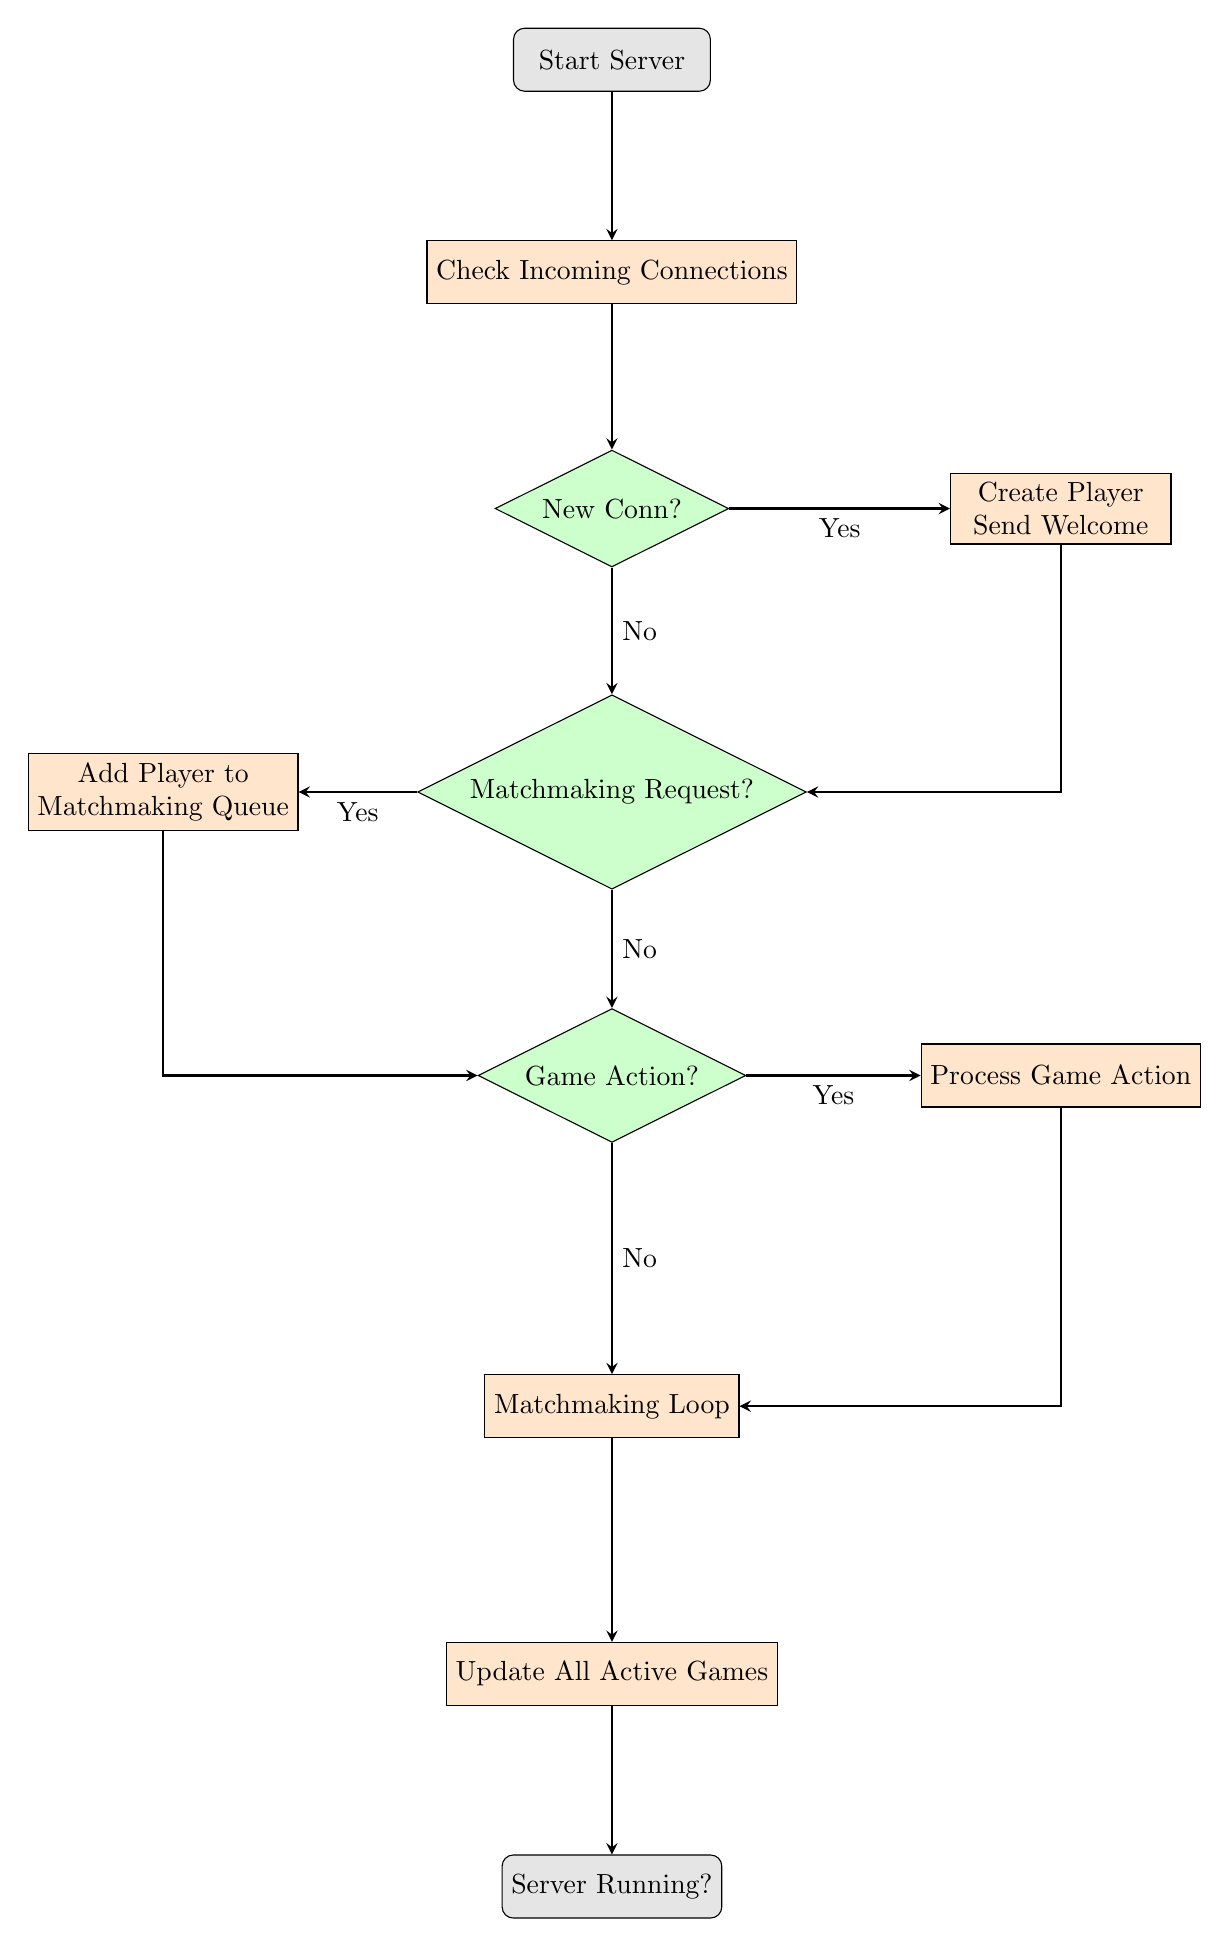
\begin{tikzpicture}[node distance=2.2cm]
\node (start) [startstop] {Start Server};
\node (conn) [process, below of=start, yshift=-0.5cm] {Check Incoming Connections};
\node (decNew) [decision, below of=conn, yshift=-0.8cm] {New Conn?};
\node (createP) [process, right of=decNew, xshift=3.5cm, align=center] {Create Player \\ Send Welcome};
\node (decMatch) [decision, below of=decNew, yshift=-1.4cm] {Matchmaking Request?};
\node (addMatch) [process, left of=decMatch, xshift=-3.5cm, align=center] {Add Player to \\ Matchmaking Queue};
\node (decGameA) [decision, below of=decMatch, yshift=-1.4cm] {Game Action?};
\node (procGameA) [process, right of=decGameA, xshift=3.5cm] {Process Game Action};
\node (matchmake) [process, below of=decGameA, yshift=-2.0cm] {Matchmaking Loop};
\node (updateGames) [process, below of=matchmake, yshift=-1.2cm] {Update All Active Games};
\node (end) [startstop, below of=updateGames, yshift=-0.5cm] {Server Running?};

\draw [arrow] (start) -- (conn);
\draw [arrow] (conn) -- (decNew);
\draw [arrow] (decNew) -- node[anchor=north] {Yes} (createP);
\draw [arrow] (decNew) -- node[anchor=west] {No} (decMatch);
\draw [arrow] (createP) |- (decMatch);
\draw [arrow] (decMatch) -- node[anchor=north] {Yes} (addMatch);
\draw [arrow] (decMatch) -- node[anchor=west] {No} (decGameA);
\draw [arrow] (addMatch) |- (decGameA);
\draw [arrow] (decGameA) -- node[anchor=north] {Yes} (procGameA);
\draw [arrow] (decGameA) -- node[anchor=west] {No} (matchmake);
\draw [arrow] (procGameA) |- (matchmake);
\draw [arrow] (matchmake) -- (updateGames);
\draw [arrow] (updateGames) -- (end);
% \draw [arrow] (end) -- ++(0,-1.0) node[anchor=north] {Yes} -| (conn);
\end{tikzpicture}%
} % end adjustbox
\caption{Main Server Loop Flowchart}
\end{figure}

\FloatBarrier

\subsubsection{Card Deployment Process Flowchart}
\begin{figure}[H]
\centering
\adjustbox{max height=0.8\textheight}{%
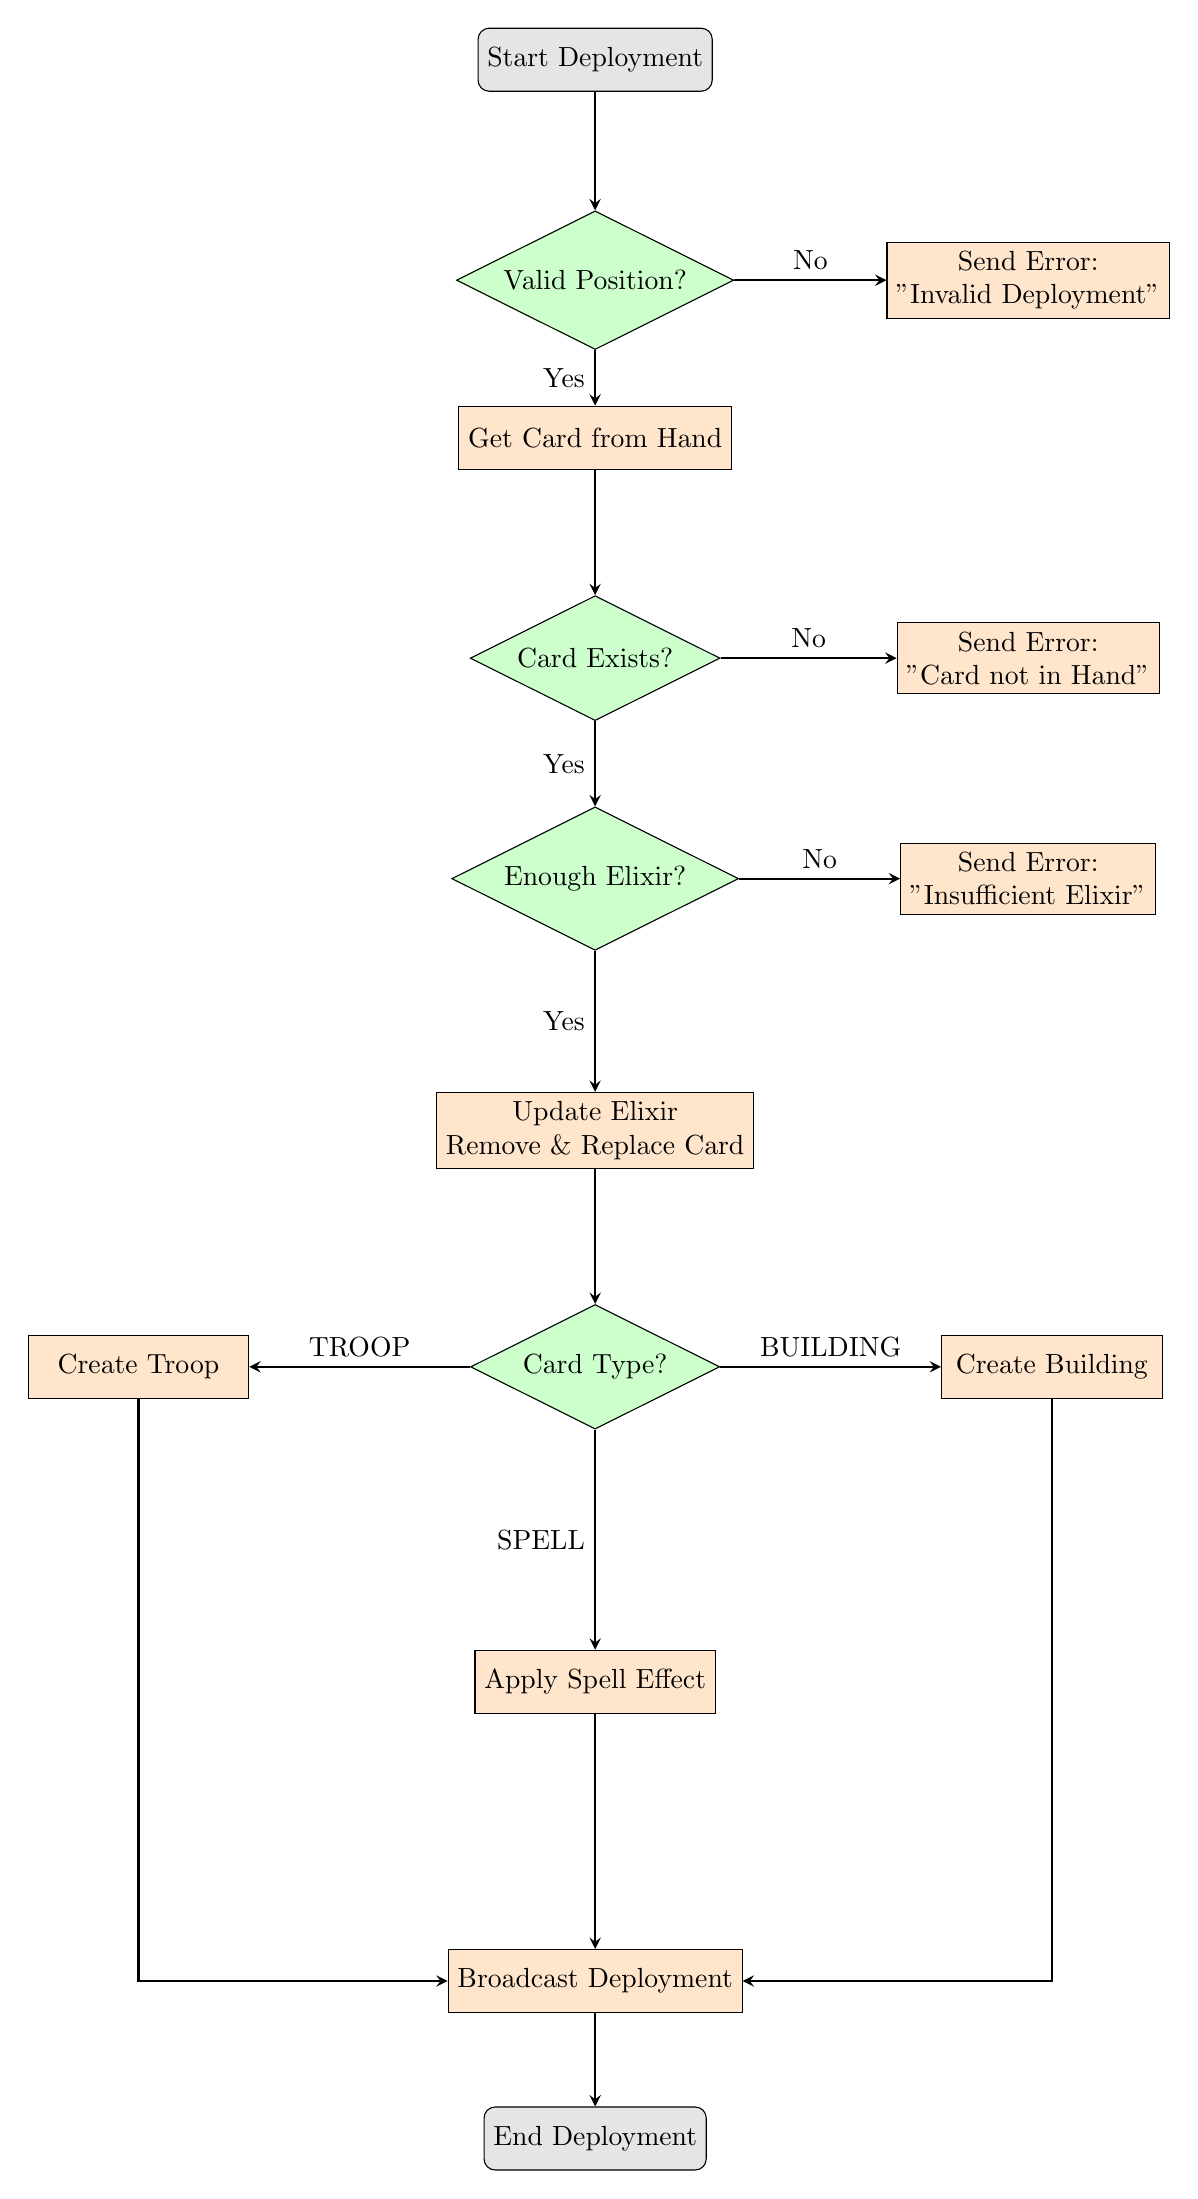
\begin{tikzpicture}[node distance=2cm]
\node (start) [startstop] {Start Deployment};
\node (checkPos) [decision, below of=start, yshift=-0.8cm] {Valid Position?};
\node (errorPos) [process, right of=checkPos, xshift=3.5cm, align=center] {Send Error: \\
"Invalid Deployment"};
\node (getCard) [process, below of=checkPos] {Get Card from Hand};
\node (cardNull) [decision, below of=getCard, yshift=-0.8cm] {Card Exists?};
\node (errorCard) [process, right of=cardNull, xshift=3.5cm, align=center] {Send Error: \\
"Card not in Hand"};
\node (checkElixir) [decision, below of=cardNull, yshift=-0.8cm] {Enough Elixir?};
\node (errorElixir) [process, right of=checkElixir, xshift=3.5cm, align=center] {Send Error: \\
"Insufficient Elixir"};
\node (deploy) [process, below of=checkElixir, yshift=-1.2cm,align=center] {Update Elixir \\
Remove \& Replace Card};
\node (typeCheck) [decision, below of=deploy, yshift=-1.0cm] {Card Type?};
\node (troop) [process, left of=typeCheck, xshift=-3.8cm] {Create Troop};
\node (spell) [process, below of=typeCheck, yshift=-2.0cm] {Apply Spell Effect};
\node (building) [process, right of=typeCheck, xshift=3.8cm] {Create Building};
\node (broadcast) [process, below of=spell, yshift=-1.8cm] {Broadcast Deployment};
\node (end) [startstop, below of=broadcast] {End Deployment};

\draw [arrow] (start) -- (checkPos);
\draw [arrow] (checkPos) -- node[anchor=east] {Yes} (getCard);
\draw [arrow] (checkPos) -- node[anchor=south] {No} (errorPos);
\draw [arrow] (getCard) -- (cardNull);
\draw [arrow] (cardNull) -- node[anchor=east] {Yes} (checkElixir);
\draw [arrow] (cardNull) -- node[anchor=south] {No} (errorCard);
\draw [arrow] (checkElixir) -- node[anchor=east] {Yes} (deploy);
\draw [arrow] (checkElixir) -- node[anchor=south] {No} (errorElixir);
\draw [arrow] (deploy) -- (typeCheck);
\draw [arrow] (typeCheck) -- node[anchor=south] {TROOP} (troop);
\draw [arrow] (typeCheck) -- node[anchor=east] {SPELL} (spell);
\draw [arrow] (typeCheck) -- node[anchor=south] {BUILDING} (building);
\draw [arrow] (troop) |- (broadcast);
\draw [arrow] (spell) -- (broadcast);
\draw [arrow] (building) |- (broadcast);
\draw [arrow] (broadcast) -- (end);
\end{tikzpicture}%
}
\caption{Card Deployment Flowchart}
\end{figure}

\FloatBarrier

\subsubsection{Battle Update Logic Flowchart}
\begin{figure}[H]
\centering
\adjustbox{max height=0.8\textheight}{%
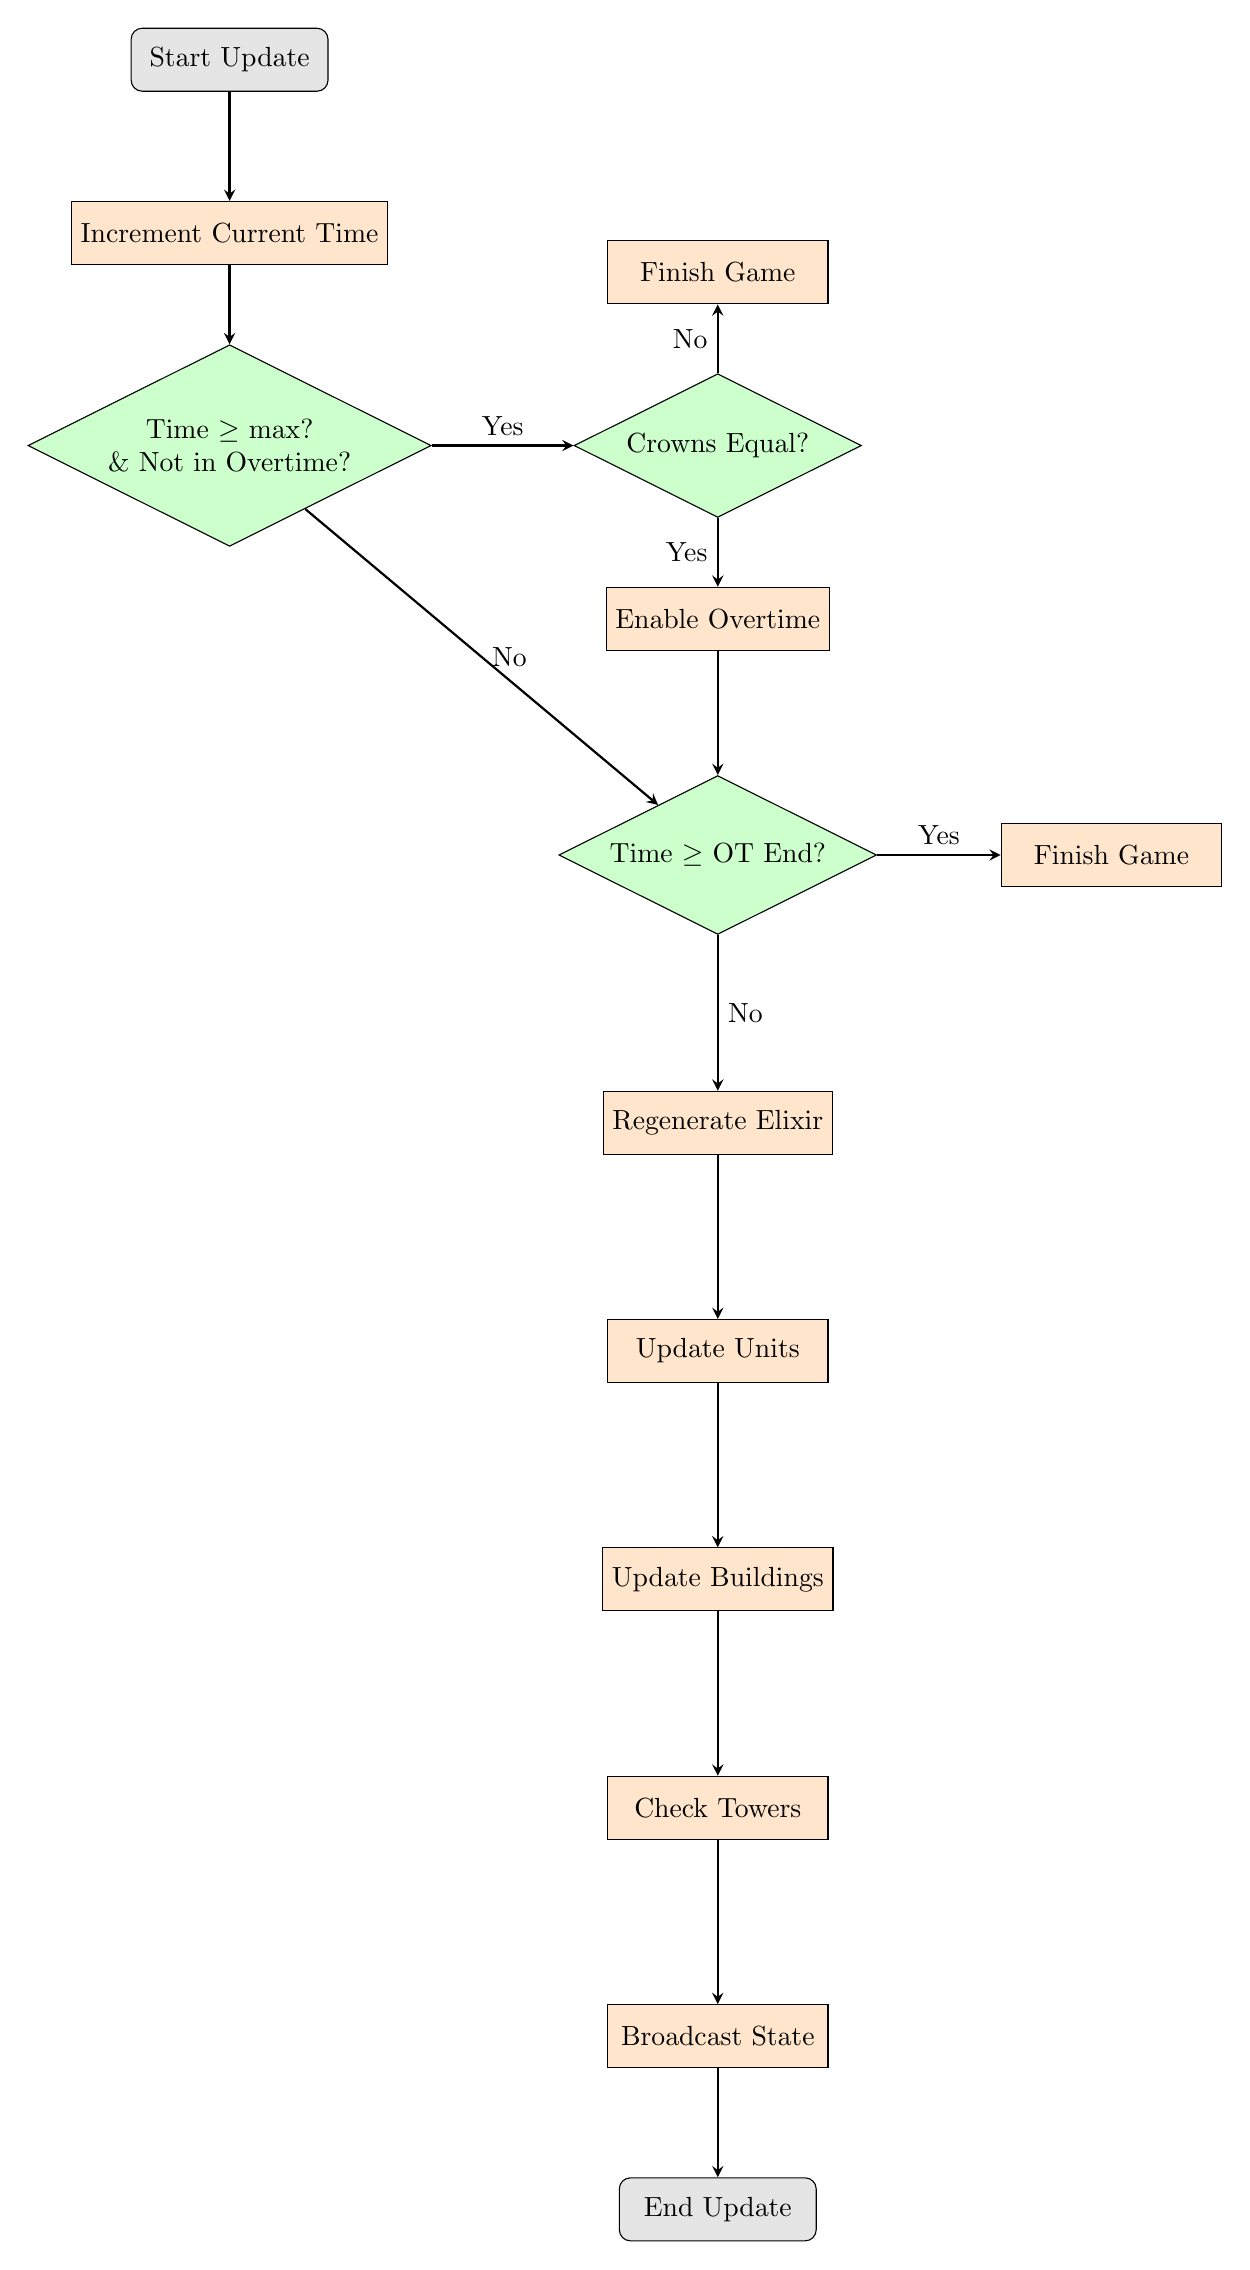
\begin{tikzpicture}[node distance=2.2cm]
\node (start) [startstop] {Start Update};
\node (timeCheck) [process, below of=start] {Increment Current Time};
\node (decOvertime) [decision, below of=timeCheck, yshift=-0.5cm,align=center] {Time $\ge$ max? \\ \& Not in Overtime?};
\node (decCrowns) [decision, right of=decOvertime, xshift=4cm] {Crowns Equal?};
\node (setOvertime) [process, below of=decCrowns] {Enable Overtime};
\node (finishGame) [process, above of=decCrowns, yshift=0.0cm] {Finish Game};
\node (otCheck) [decision, below of=setOvertime, yshift=-0.8cm] {Time $\ge$ OT End?};
\node (finishGame2) [process, right of=otCheck, xshift=2.8cm] {Finish Game};
\node (regen) [process, below of=otCheck, yshift=-1.2cm] {Regenerate Elixir};
\node (units) [process, below of=regen, yshift=-0.7cm] {Update Units};
\node (buildings) [process, below of=units, yshift=-0.7cm] {Update Buildings};
\node (checkTowers) [process, below of=buildings, yshift=-0.7cm] {Check Towers};
\node (broadcast) [process, below of=checkTowers, yshift=-0.7cm] {Broadcast State};
\node (end) [startstop, below of=broadcast] {End Update};

\draw [arrow] (start) -- (timeCheck);
\draw [arrow] (timeCheck) -- (decOvertime);
\draw [arrow] (decOvertime) -- node[anchor=south] {Yes} (decCrowns);
\draw [arrow] (decOvertime) -- node[anchor=west] {No} (otCheck);
\draw [arrow] (decCrowns) -- node[anchor=east] {Yes} (setOvertime);
\draw [arrow] (decCrowns) -- node[anchor=east] {No} (finishGame);
\draw [arrow] (setOvertime) -- (otCheck);
\draw [arrow] (otCheck) -- node[anchor=south] {Yes} (finishGame2);
\draw [arrow] (otCheck) -- node[anchor=west] {No} (regen);
\draw [arrow] (regen) -- (units);
\draw [arrow] (units) -- (buildings);
\draw [arrow] (buildings) -- (checkTowers);
\draw [arrow] (checkTowers) -- (broadcast);
\draw [arrow] (broadcast) -- (end);
\end{tikzpicture}%
}
\caption{Battle Update Logic Flowchart}
\end{figure}

\FloatBarrier

\subsubsection{Target Selection Algorithm Flowchart}
\begin{figure}[H]
\centering
\adjustbox{max height=0.8\textheight}{%
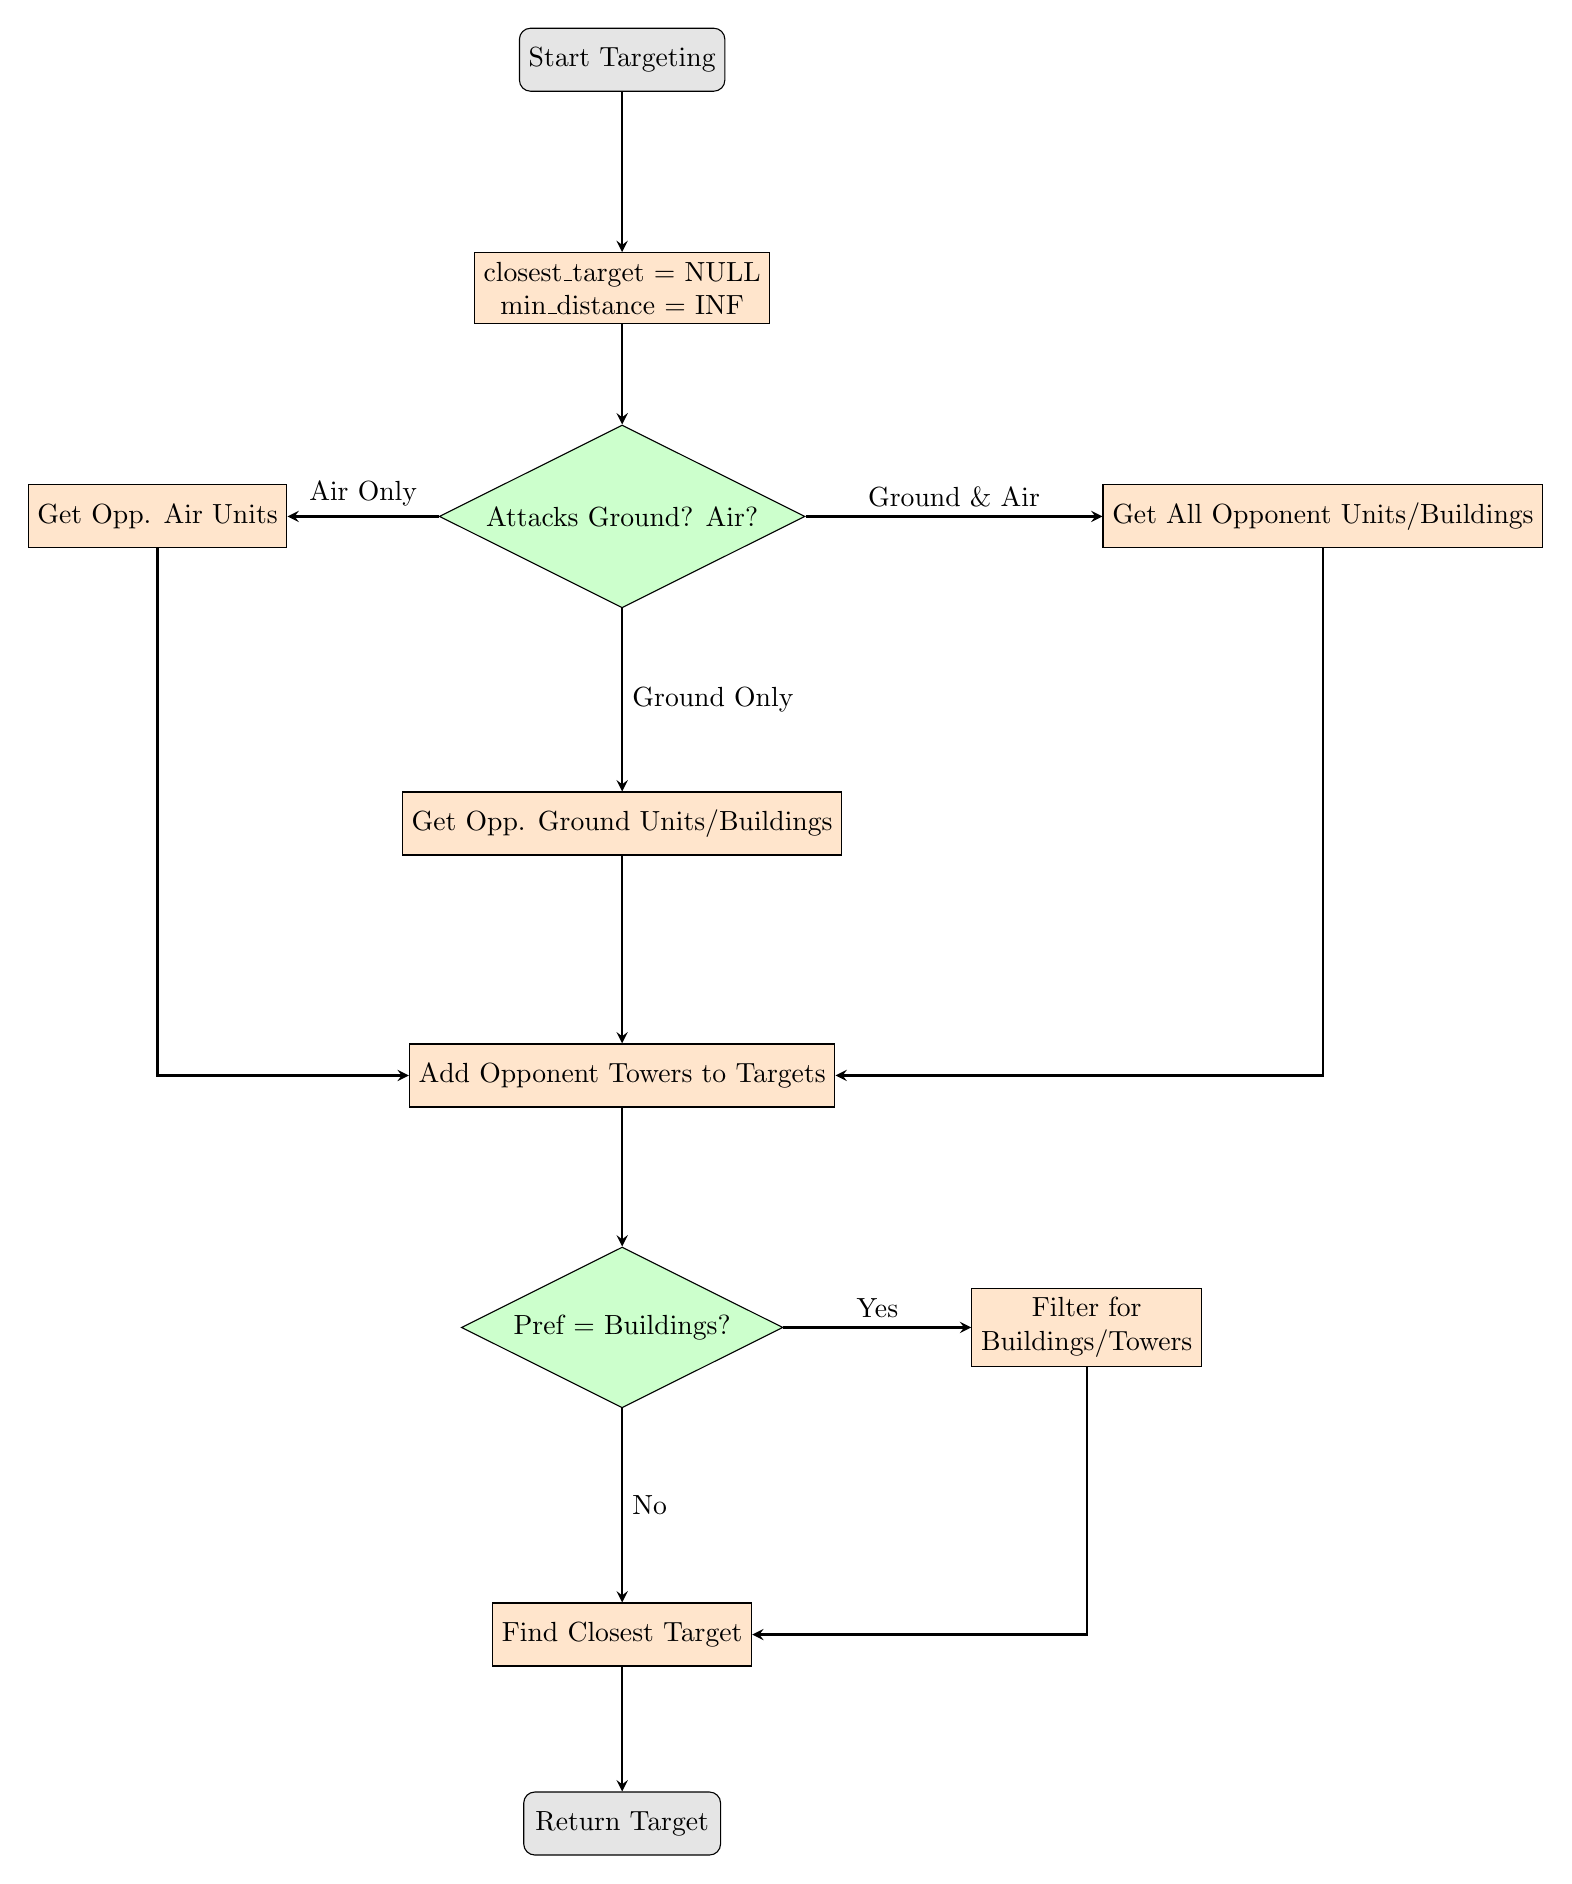
\begin{tikzpicture}[node distance=2.4cm]
\node (start) [startstop] {Start Targeting};
\node (initVar) [process, below of=start, yshift=-0.5cm,align=center] {closest\_target = NULL \\ min\_distance = INF};
\node (attType) [decision, below of=initVar, yshift=-0.5cm] {Attacks Ground? Air?};
\node (getAll) [process, right of=attType, xshift=6.5cm] {Get All Opponent Units/Buildings};
\node (getGround) [process, below of=attType, yshift=-1.5cm] {Get Opp. Ground Units/Buildings};
\node (getAir) [process, left of=attType, xshift=-3.5cm] {Get Opp. Air Units};
\node (addTowers) [process, below of=getGround, yshift=-0.8cm] {Add Opponent Towers to Targets};
\node (pref) [decision, below of=addTowers, yshift=-0.8cm] {Pref = Buildings?};
\node (filterBld) [process, right of=pref, xshift=3.5cm,align=center] {Filter for \\ Buildings/Towers};
\node (loopTargets) [process, below of=pref, yshift=-1.5cm] {Find Closest Target};
\node (end) [startstop, below of=loopTargets] {Return Target};

\draw [arrow] (start) -- (initVar);
\draw [arrow] (initVar) -- (attType);
\draw [arrow] (attType) -- node[anchor=south] {Ground \& Air} (getAll);
\draw [arrow] (attType) -- node[anchor=west] {Ground Only} (getGround);
\draw [arrow] (attType) -- node[anchor=south] {Air Only} (getAir);
\draw [arrow] (getAir) |- (addTowers);
\draw [arrow] (getGround) -- (addTowers);
\draw [arrow] (getAll) |- (addTowers);
\draw [arrow] (addTowers) -- (pref);
\draw [arrow] (pref) -- node[anchor=south] {Yes} (filterBld);
\draw [arrow] (filterBld) |- (loopTargets);
\draw [arrow] (pref) -- node[anchor=west] {No} (loopTargets);
\draw [arrow] (loopTargets) -- (end);
\end{tikzpicture}%
}
\caption{Target Selection Flowchart}
\end{figure}

\FloatBarrier

\subsubsection{Chest Reward System Flowchart}
\begin{figure}[H]
\centering
\adjustbox{max height=0.8\textheight}{%
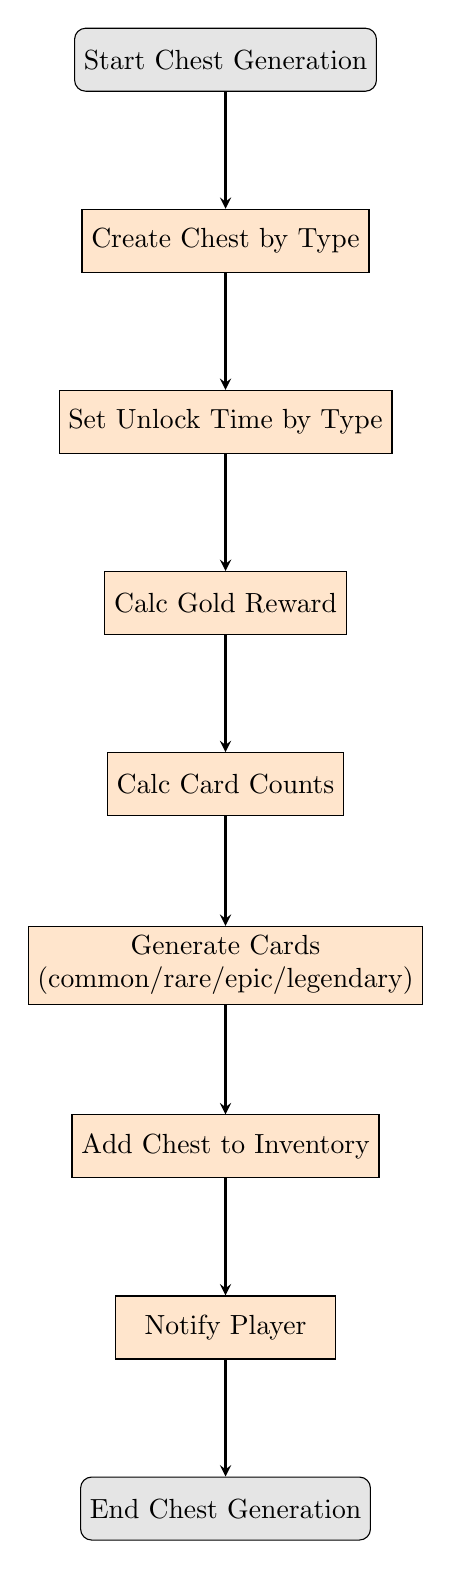
\begin{tikzpicture}[node distance=2.3cm]
\node (start) [startstop] {Start Chest Generation};
\node (createC) [process, below of=start] {Create Chest by Type};
\node (setTime) [process, below of=createC] {Set Unlock Time by Type};
\node (gold) [process, below of=setTime] {Calc Gold Reward};
\node (cards) [process, below of=gold] {Calc Card Counts};
\node (generate) [process, below of=cards, align=center] {Generate Cards \\ (common/rare/epic/legendary)};
\node (addChest) [process, below of=generate] {Add Chest to Inventory};
\node (notify) [process, below of=addChest] {Notify Player};
\node (end) [startstop, below of=notify] {End Chest Generation};

\draw [arrow] (start) -- (createC);
\draw [arrow] (createC) -- (setTime);
\draw [arrow] (setTime) -- (gold);
\draw [arrow] (gold) -- (cards);
\draw [arrow] (cards) -- (generate);
\draw [arrow] (generate) -- (addChest);
\draw [arrow] (addChest) -- (notify);
\draw [arrow] (notify) -- (end);
\end{tikzpicture}%
}
\caption{Chest Reward System Flowchart}
\end{figure}

\FloatBarrier

\section{Trace Tables}
The following subsections provide example trace tables for typical scenarios in each major workflow.

\subsection{Main Server Loop Trace Table}
\begin{table}[H]
\centering
\footnotesize
\begin{tabular}{|c|p{3.2cm}|p{4cm}|p{2.5cm}|p{2.5cm}|}
\hline
\textbf{Step} & \textbf{Condition} & \textbf{Action} & \textbf{player\_registry} & \textbf{active\_games} \\
\hline
1 & new\_connections=[ConnA] & REGISTER\_PLAYER(ConnA) & \{1: PlayerA\} & \{\} \\
\hline
2 & PlayerA requests matchmaking & matchmaking\_queue.ADD(PlayerA) & \{1: PlayerA\} & \{\} \\
\hline
3 & new\_connections=[ConnB] & REGISTER\_PLAYER(ConnB) & \{1: PlayerA, 2: PlayerB\} & \{\} \\
\hline
4 & PlayerB requests matchmaking & matchmaking\_queue.ADD(PlayerB) & same & \{\} \\
\hline
5 & PROCESS\_MATCHMAKING finds pair & INITIALIZE\_NEW\_GAME & same & \{1001: Game1\} \\
\hline
6 & event\_dispatcher.EXECUTE & no pending events & same & same \\
\hline
\end{tabular}
\caption{Main Server Loop - Two Players Matching}
\end{table}

\subsection{Player Handling (HANDLE\_PLAYER) Trace Table}
\begin{table}[H]
\centering
\footnotesize
\begin{tabular}{|c|p{4cm}|p{4cm}|p{2.5cm}|}
\hline
\textbf{Step} & \textbf{Condition} & \textbf{Action} & \textbf{Outcome}\\
\hline
1 & player.is\_active = True & WAIT\_FOR\_REQUEST() & request = None \\
\hline
2 & request is None & loop repeats & handle\_player in wait \\
\hline
3 & external event: player.is\_active=False & exit loop & CLEANUP\_PLAYER(player) \\
\hline
4 & CLEANUP\_PLAYER & close socket, remove from queue & player inactivated \\
\hline
\end{tabular}
\caption{HANDLE\_PLAYER - Disconnect Scenario}
\end{table}

\subsection{Request Routing (HANDLE\_PLAYER\_REQUEST) Trace Table}
\begin{table}[H]
\centering
\footnotesize
\begin{tabular}{|c|p{3.5cm}|p{4cm}|p{2.5cm}|}
\hline
\textbf{Step} & \textbf{Input} & \textbf{Check / Action} & \textbf{Outcome}\\
\hline
1 & request.type="game\_action" & GET\_ACTIVE\_GAME\_FOR\_PLAYER & game=Game1 \\
\hline
2 & action="deploy", card\_id="knight" & ProcessCardDeployment & successful deployment \\
\hline
3 & else branch? & not triggered & - \\
\hline
4 & End & - & Request done \\
\hline
\end{tabular}
\caption{Request Routing - Deploy Action}
\end{table}

\subsection{Matchmaking Process Trace Table}
\begin{table}[H]
\centering
\footnotesize
\begin{tabular}{|c|p{3.5cm}|p{4cm}|p{2.5cm}|p{2.5cm}|}
\hline
\textbf{Step} & \textbf{Condition} & \textbf{Action} & \textbf{matchmaking\_queue} & \textbf{active\_games} \\
\hline
1 & queue.has\_pairs()=True & get\_matched\_players() & empty after pop & \{\} \\
\hline
2 & players valid & initialize new game & [] & \{2001: GameObj\} \\
\hline
3 & queue.has\_pairs()=False & break & [] & same \\
\hline
\end{tabular}
\caption{Matchmaking - Single Pair Scenario}
\end{table}

\subsection{Game Update Thread (UpdateAllGames) Trace Table}
\begin{table}[H]
\centering
\footnotesize
\begin{tabular}{|c|p{3.5cm}|p{3.5cm}|p{3cm}|p{3cm}|}
\hline
\textbf{Step} & \textbf{Games} & \textbf{Check} & \textbf{Action} & \textbf{Result}\\
\hline
1 & \{G1(not terminated), G2(terminated)\} & G1: not terminated & G1.UPDATE() & G1 remains active \\
\hline
2 & G2: is\_terminated=True & remove from active\_games & G2 removed & \{G1\} left \\
\hline
3 & Sleep & 1 / TICK\_RATE & wait next frame & - \\
\hline
\end{tabular}
\caption{Game Update Thread - One Terminated, One Active}
\end{table}

\subsection{Game Update Logic (UPDATE\_GAME) Trace Table}
\begin{table}[H]
\centering
\footnotesize
\begin{tabular}{|c|p{3cm}|p{5cm}|p{3cm}|}
\hline
\textbf{Step} & \textbf{Condition} & \textbf{Action} & \textbf{Outcome}\\
\hline
1 & time\_elapsed=179, max\_duration=180 & INCREMENT\_TIME(1s) & time\_elapsed=180 \\
\hline
2 & check\_end\_conditions & time\_elapsed >= 180 & DETERMINE\_GAME\_WINNER\_BY\_HP, TERMINATE \\
\hline
3 & after termination & skip further steps & game ended \\
\hline
\end{tabular}
\caption{Game Update Logic - Timeout Scenario}
\end{table}

\subsection{Card Deployment Process Trace Table}
\begin{table}[H]
\centering
\footnotesize
\begin{tabular}{|c|p{3.5cm}|p{4cm}|p{3cm}|}
\hline
\textbf{Step} & \textbf{Condition} & \textbf{Action} & \textbf{Result}\\
\hline
1 & position=(3,4) & VALIDATE\_DEPLOYMENT\_POSITION & valid position \\
\hline
2 & card in hand & yes & proceed \\
\hline
3 & player.elixir=6, cost=4 & verify cost & enough elixir \\
\hline
4 & SPEND\_ELIXIR(4) & discard card, draw next & elixir=2 \\
\hline
5 & CREATE\_ENTITY & new troop in game & entity registered \\
\hline
6 & BROADCAST\_DEPLOYMENT & all players see new troop & done \\
\hline
\end{tabular}
\caption{Card Deployment - Valid Scenario}
\end{table}

\subsection{Target Selection Algorithm Trace Table}
\begin{table}[H]
\centering
\footnotesize
\begin{tabular}{|c|p{3.5cm}|p{4cm}|p{3.5cm}|}
\hline
\textbf{Step} & \textbf{Targets} & \textbf{Compute Score} & \textbf{Min Score Target}\\
\hline
1 & [T1, T2, T3] & T1=10, T2=7, T3=12 & T2 is best so far \\
\hline
2 & best\_target = T2 & - & final = T2 \\
\hline
\end{tabular}
\caption{Target Selection - Closest Target Example}
\end{table}

\subsection{Chest Reward System Trace Table}
\begin{table}[H]
\centering
\footnotesize
\begin{tabular}{|c|p{3.5cm}|p{5cm}|p{3cm}|}
\hline
\textbf{Step} & \textbf{Input} & \textbf{Action} & \textbf{Outcome}\\
\hline
1 & chest\_type="gold" & CREATE\_CHEST\_INSTANCE("gold") & chest.type=gold \\
\hline
2 & ASSIGN\_UNLOCK\_TIME & 8 hours & chest.unlock\_time=28800 \\
\hline
3 & ALLOCATE\_GOLD\_REWARDS & base=100+(arena*10) & added to chest \\
\hline
4 & ALLOCATE\_CARD\_REWARDS & \{common:20, rare:5, epic:1\} & random picks \\
\hline
5 & INCREMENT\_CHEST\_COLLECTION & chest added to inventory & player has new chest \\
\hline
6 & SEND\_REWARD\_NOTIFICATION & player alerted & done \\
\hline
\end{tabular}
\caption{Chest Reward System - Gold Chest Scenario}
\end{table}
\end{document}
